\documentclass[a4paper,10pt]{article}
\usepackage{multicol}
% ---------- 页面布局/基础配置 ----------
\usepackage{geometry}
\geometry{left=1in,right=0.75in,top=0.9in,bottom=0.9in}
\usepackage{microtype}

% ---------- 编码/字体 ----------
\usepackage[T1]{fontenc}
\usepackage[utf8]{inputenc}
\usepackage[table]{xcolor}
\usepackage{newtxtext}
\usepackage{amsmath, amssymb, amsthm}
\usepackage{newtxmath}
\usepackage{mathtools}
\usepackage{bm}
\usepackage{esint}

% 计算机/算法
\usepackage{algorithm}
\usepackage{algpseudocode}
\algnewcommand{\Initialize}{\State\textbf{Initialize:}}

% .md转.tex
\providecommand{\tightlist}{\setlength{\itemsep}{0pt}\setlength{\parskip}{0pt}}
\usepackage{longtable}
\usepackage{fvextra}

% 单位
\usepackage{siunitx}
\sisetup{unit-mode=text}
\newcommand{\vect}[1]{\vec{#1}}
\newcommand{\Vect}[1]{\overrightarrow{#1}}
\newcommand{\grad}{\nabla}
\newcommand{\degree}{^\circ}

% 自定义命令
\newcommand{\pd}[2]{\dfrac{\partial #1}{\partial #2}}
\newcommand{\PD}[2]{\frac{\partial #1}{\partial #2}}
\newcommand{\eq}[1]{Eq.\ (\ref{#1})}
\newcommand{\fig}[1]{Figure~\ref{#1}}
\newcommand{\tab}[1]{Table~\ref{#1}}

% 数学
\newcommand{\dd}{\mathrm{d}}
\newcommand{\dx}{\,\mathrm{d}x}
\newcommand{\limit}[2]{\lim_{#1 \to #2}}
\newcommand{\pard}[2]{\frac{\partial #1}{\partial #2}}

% 线性代数
\newcommand{\R}{\mathbb{R}}
\newcommand{\C}{\mathbb{C}}
\newcommand{\N}{\mathbb{N}}
\newcommand{\bvec}[1]{\mathbf{#1}}
\newcommand{\mat}[1]{\begin{bmatrix}#1\end{bmatrix}}
\newcommand{\pmat}[1]{\begin{pmatrix}#1\end{pmatrix}}
\newcommand{\trans}{^\top}
\newcommand{\inv}{^{-1}}
\DeclareMathOperator{\rank}{rank}
\DeclareMathOperator{\tr}{tr}
\DeclareMathOperator{\spanop}{span}

% 统计学
\newcommand{\Prob}[1]{P\left(#1\right)}
\newcommand{\Exp}[1]{E\left[#1\right]}
\newcommand{\Var}[1]{\text{Var}\left(#1\right)}
\newcommand{\Cov}[1]{\text{Cov}\left(#1\right)}
\newcommand{\indep}{\perp\!\!\!\perp}
\newcommand{\Norm}{\mathcal{N}}
\newcommand{\Bin}{\text{Bin}}
\newcommand{\Poi}{\text{Pois}}
\newcommand{\yhat}{\hat{y}}
\newcommand{\betahat}{\hat{\beta}}

% 页面排版
\usepackage{titling}
\usepackage{titlesec}
\usepackage{float}
\usepackage{lipsum}
\usepackage{enumitem}
\usepackage{caption}
\usepackage{subcaption}
\usepackage{tabularx}
\newcolumntype{Y}{>{\raggedright\arraybackslash}X}
\usepackage{setspace}
\usepackage{fancyhdr}
\usepackage{url}
\usepackage{hyperref}
\usepackage{booktabs}
\usepackage{array}
\usepackage{multirow}
\usepackage{pdflscape}
\usepackage{pdfpages}

% 代码块
\usepackage{listings}
\usepackage{mdframed}
\usepackage[numbers]{natbib}
\lstset{
    basicstyle=\small\ttfamily,
    breaklines=true,
    breakatwhitespace=false,
    backgroundcolor=\color{gray!5},
    frame=single,
    framesep=3pt,
    xleftmargin=5pt,
    xrightmargin=5pt,
    lineskip=0.5pt,
    showstringspaces=false
}

% 画图
\usepackage{graphicx}
\usepackage{tikz}
\usepackage{pgfplots}
\pgfplotsset{compat=1.18}

% 颜色
\usepackage{xcolor}
\definecolor{refblue}{HTML}{A3C4F3}
\definecolor{repgreen}{HTML}{C8E6C9}
\definecolor{transorange}{HTML}{FFD54F}
\definecolor{subviolet}{HTML}{E1BEE7}
\definecolor{ellipgray}{HTML}{E0E0E0}
\newcommand{\refhl}[1]{\sethlcolor{refblue}\hl{#1}}
\newcommand{\rephl}[1]{\sethlcolor{repgreen}\hl{#1}}
\newcommand{\transhl}[1]{\sethlcolor{transorange}\hl{#1}}
\newcommand{\subhl}[1]{\sethlcolor{subviolet}\hl{#1}}
\newcommand{\elliphl}[1]{\sethlcolor{ellipgray}\hl{#1}}

\usepackage{tcolorbox}
\tcbuselibrary{breakable,skins}
\hypersetup{
    colorlinks=true,
    linkcolor=blue,
    citecolor=blue,
    urlcolor=blue,
    pdfborder={0 0 0}
}

\newtheorem{theorem}{Theorem}
\newtheorem{definition}{Definition}

% ==================== 文档开始 ======================
\begin{document}
\title{UFUG 2104 \\[4pt] Assignment 1: Project Report}
\author{Jincan LI}
\date{\today}
\maketitle

% ==================== 1. Introduction ======================
\section{Introduction}\label{sec:intro}

\subsection{Dataset Overview}
This project analyzes the \textit{Billionaires Statistics Dataset (2023)}, a cross-sectional snapshot of $n=2{,}640$ records capturing the world's wealthiest individuals.
Each record carries 35 raw variables spanning wealth metrics (\texttt{finalWorth}), personal demographics (\texttt{age}, \texttt{gender}, \texttt{selfMade}), geographic identifiers (\texttt{country}, \texttt{city}), business information (\texttt{category}, \texttt{source}, \texttt{organization}), and country-level macroeconomic indicators (\texttt{gdp\_country}, \texttt{population\_country}, \texttt{life\_expectancy\_country}, etc.).
All monetary values are in millions of USD.

\subsection{Research Context and Theoretical Framing}

\textbf{Why billionaire wealth is a window into economic inequality.}
The distribution of billionaire wealth is not merely a curiosity---it sits at the intersection of several major economic debates: the measurement of inequality (Pareto's law \cite{pareto1896}, the Gini coefficient \cite{cowell2011}), the mechanisms of capital accumulation (Romer's endogenous growth theory \cite{romer1990}, Piketty's $r>g$ framework \cite{piketty2014}), and the empirical study of whether national prosperity translates into broad-based wealth creation.

\textbf{Three analytical layers drive this report:}
\begin{enumerate}
    \item \textbf{The tail-layer problem}: Billionaire wealth lives in the extreme upper tail of the global wealth distribution, where standard statistical methods (arithmetic mean, variance-based tests, raw-scale OLS) can be dominated by a handful of observations. This motivates log transforms, non-parametric methods, and robust inference.
    \item \textbf{The association vs. causation problem}: Correlations between national GDP and individual billionaire wealth are inherently observational. The analysis estimates the \emph{conditional association} (not causal effect) of macroeconomic context with individual wealth, while acknowledging confounders such as capital market depth, institutional quality, tax regimes, and family network density.
    \item \textbf{The heterogeneity problem}: Aggregate correlations obscure substantial heterogeneity across industries and wealth-accumulation paths. A single pooled estimate may be simultaneously uninterpretable for an entrepreneur in Shenzhen and misleading for a fashion billionaire in Milan.
\end{enumerate}

These three layers structure the narrative arc of this report: first diagnosing the heavy-tailed distribution, then quantifying associations with uncertainty, and finally testing whether those associations hold across subgroups and under alternative specifications.

\subsection{Research Questions}
Table~\ref{tab:rq} presents the seven research questions that structure this report.

\begin{table}[H]
\centering
\caption{Research questions and their mapping to analytical modules.}
\label{tab:rq}
\scriptsize
\resizebox{\textwidth}{!}{\input{output/tab/tab_M0_research_questions.tex}}
\end{table}

\subsection{Analytical Logic Chain}
The report follows a deliberately ordered evidence chain rather than a flat catalogue of outputs.
First, the raw file is frozen and its record logic is checked, because duplicated aliases, structural missingness, and country-level macro variables determine what can be modeled responsibly.
Second, the outcome distribution is diagnosed before inference; the heavy right tail justifies log-scale visualization, rank-based correlations, bootstrap intervals, and robust standard errors.
Third, descriptive geography and industry summaries are used to understand composition, not to infer population prevalence.
Fourth, inferential tests are interpreted through effect sizes and uncertainty rather than through $p$-values alone.
Finally, regression and robustness checks test whether the headline associations survive changes in scale, sample definition, and subgroup structure.

This ordering matters for the substantive claims: the report does not start by asking whether GDP ``explains'' billionaire wealth. It first asks whether the dataset is stable enough to analyze, whether the outcome is too heavy-tailed for ordinary methods, and whether pooled associations hide industry or pathway heterogeneity. Only after those checks does the regression section estimate GDP elasticity.

\bigskip

% ==================== 2. Statistical Analysis ======================
\section{Statistical Analysis}\label{sec:stats}

% --- 2.1 Data Processing ---
\subsection{Data Governance: Schema Freeze, Missingness Architecture, and the Logic of Cleaning}\label{sec:data}

\subsubsection{Schema Freeze: Treating Raw Data as Immutable Infrastructure}
The analysis uses a schema-freeze discipline: the raw CSV is never modified in-place. All transformations produce derived columns, and every change is logged with a timestamp, field name, old value, new value, and rationale.

\textbf{Schema fingerprint:} SHA-256
{\scriptsize\texttt{af398e929329cc44166e04ab763243de50d0bf049974a0b8c2544ba2db21760e}};
shape at ingest: $2{,}640 \times 35$.
CSV read command:
\begin{verbatim}
pd.read_csv(PATH, encoding='utf-8', na_values=['', 'N/A', 'None', '?'])
\end{verbatim}
No records were deleted; all $2{,}640$ observations are preserved in the cleaned dataset.

\textbf{Primary variables (P0) for this analysis:} \texttt{finalWorth}, \texttt{gdp\_country}, \texttt{selfMade}, \texttt{gender}, \texttt{category}, \texttt{country}, \texttt{age}.

Figure~\ref{fig:varroles} summarizes the variable triage step that precedes modeling. It is included because the earlier exploratory draft's strongest contribution was not only its results, but also its explicit reasoning about which fields should be modeled, which should be used descriptively, and which should be excluded from primary inference.

\begin{figure}[H]
\centering
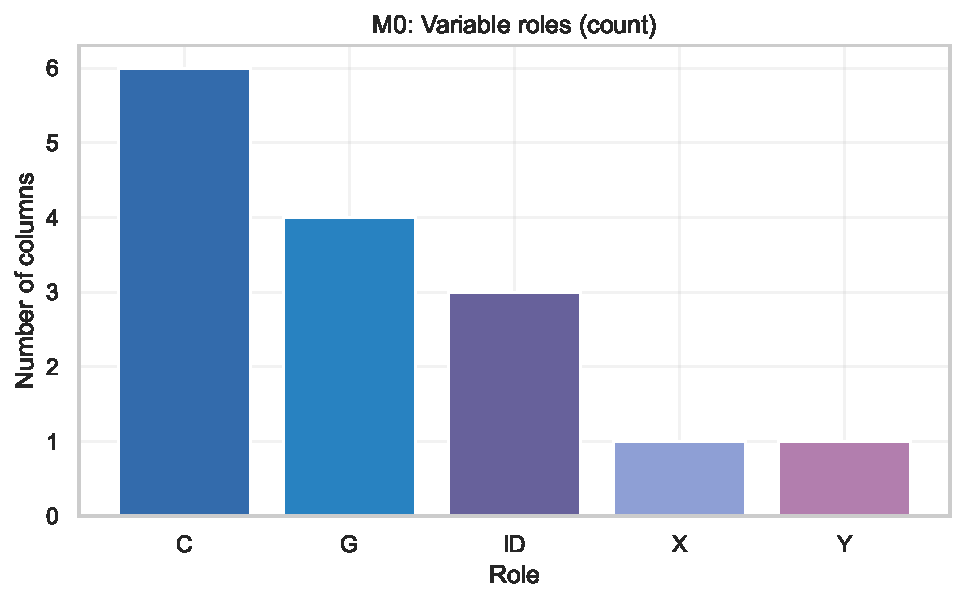
\includegraphics[width=0.68\linewidth]{output/fig/fig_M0_variable_role_counts.pdf}
\caption{Variable-role triage before modeling. The primary model uses a small core of defensible variables; other fields are retained as descriptive context, audit variables, or excluded metadata.}
\label{fig:varroles}
\end{figure}

Before modeling, the data structure requires several identity checks. The field \texttt{personName} is not a stable primary key; \texttt{category} and \texttt{industries} are exact aliases; \texttt{date} is snapshot metadata rather than a time-series variable; and \texttt{(rank, country, personName)} is only a snapshot-level surrogate key. Table~\ref{tab:identityaudit} summarizes these checks. They matter because the dataset contains descriptive labels and repeated country-level fields that should not be treated as independent individual-level measurements.

\begin{table}[H]
\centering
\caption{Record identity and alias checks before modeling.}
\label{tab:identityaudit}
\scriptsize
\resizebox{\textwidth}{!}{\input{output/tab/tab_M1_identity_audit.tex}}
\end{table}

\subsubsection{Missingness Architecture: Three Distinct Patterns}
Missingness is characterized not merely as a percentage, but as a \emph{pattern} that carries structural information about how the dataset was assembled.

\textbf{Pattern 1 -- Structural missingness (U.S.-only fields):}
\texttt{state} and \texttt{residenceStateRegion} are populated exclusively for U.S. citizens. All non-U.S. records show 100\% missingness in these columns by design. Treating this as a data-quality problem would be a category error.

\textbf{Pattern 2 -- Country-level macro linkage:}
Macroeconomic variables (GDP, CPI, life expectancy, tax revenue, etc.) share a common missingness mechanism: they are fetched via an ISO country-code lookup. If a \texttt{country} value does not match the lookup table, all macro variables for that person are simultaneously \texttt{NaN}. This creates \emph{clustered} missingness concentrated in countries with non-standard naming conventions in the dataset.

\textbf{Pattern 3 -- Sparse identifiers:}
\texttt{organization} (87.7\% missing) and \texttt{title} (87.2\% missing) are populated only for publicly listed or widely documented individuals. Their absence is structurally informative (small/private businesses are less visible), and these fields are not used in any primary analysis.

Figure~\ref{fig:usstate} documents Pattern 1; Figure~\ref{fig:miss15} shows the top-15 missingness rates; Figure~\ref{fig:missheat} shows the country-level clustering of macro missingness.

\begin{figure}[H]
\centering
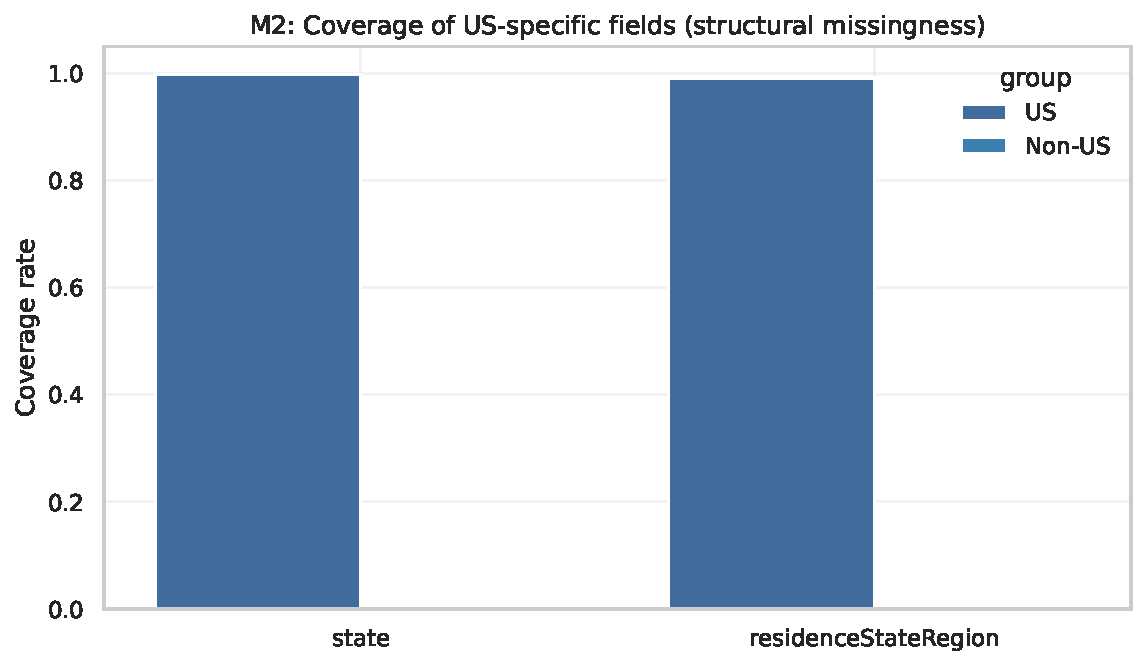
\includegraphics[width=0.88\linewidth]{output/fig/fig_M2_us_only_state_coverage.pdf}
\caption{Structural coverage: state/region fields are populated only for U.S. records (100\% missing for non-U.S.). This is a design artifact, not a data quality defect.}
\label{fig:usstate}
\end{figure}

\begin{figure}[H]
\centering
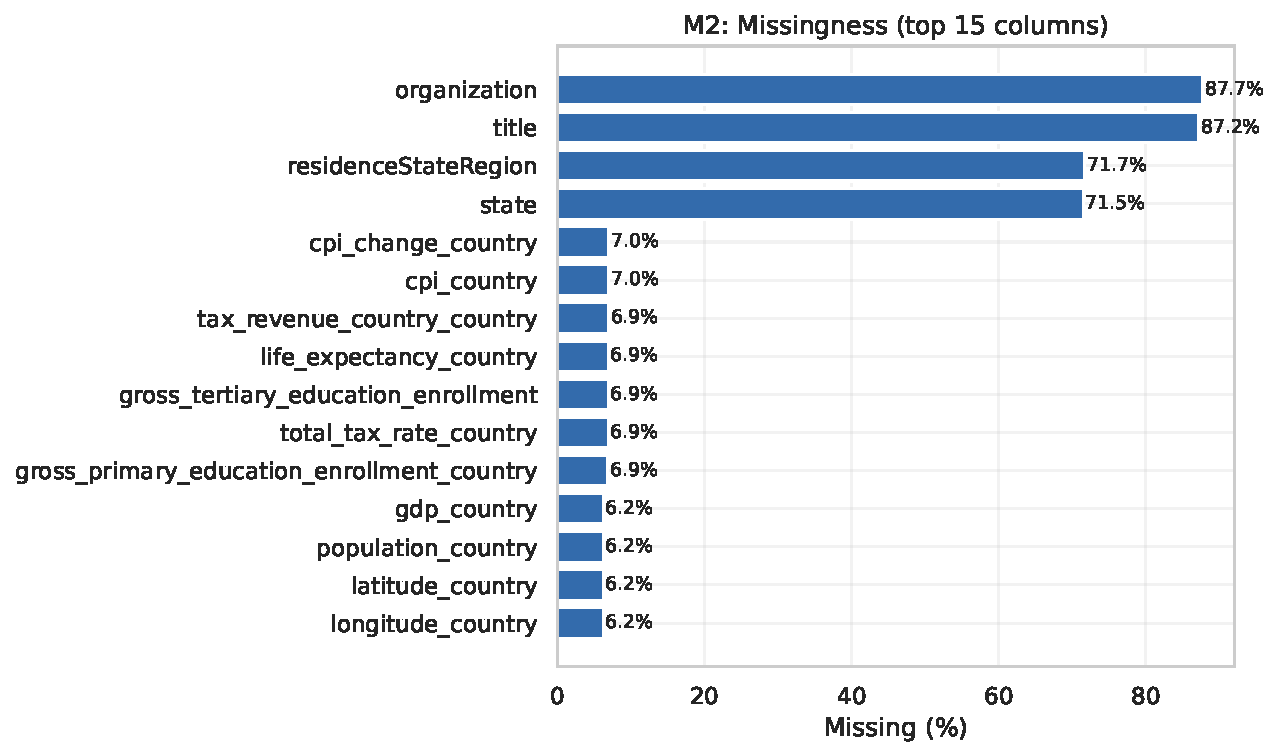
\includegraphics[width=0.86\linewidth]{output/fig/fig_M2_missingness_top15.pdf}
\caption{Top-15 variables by missingness rate. Variables \texttt{organization} and \texttt{title} exceed 87\% missingness; macro variables cluster at 6--7\%.}
\label{fig:miss15}
\end{figure}

\begin{figure}[H]
\centering
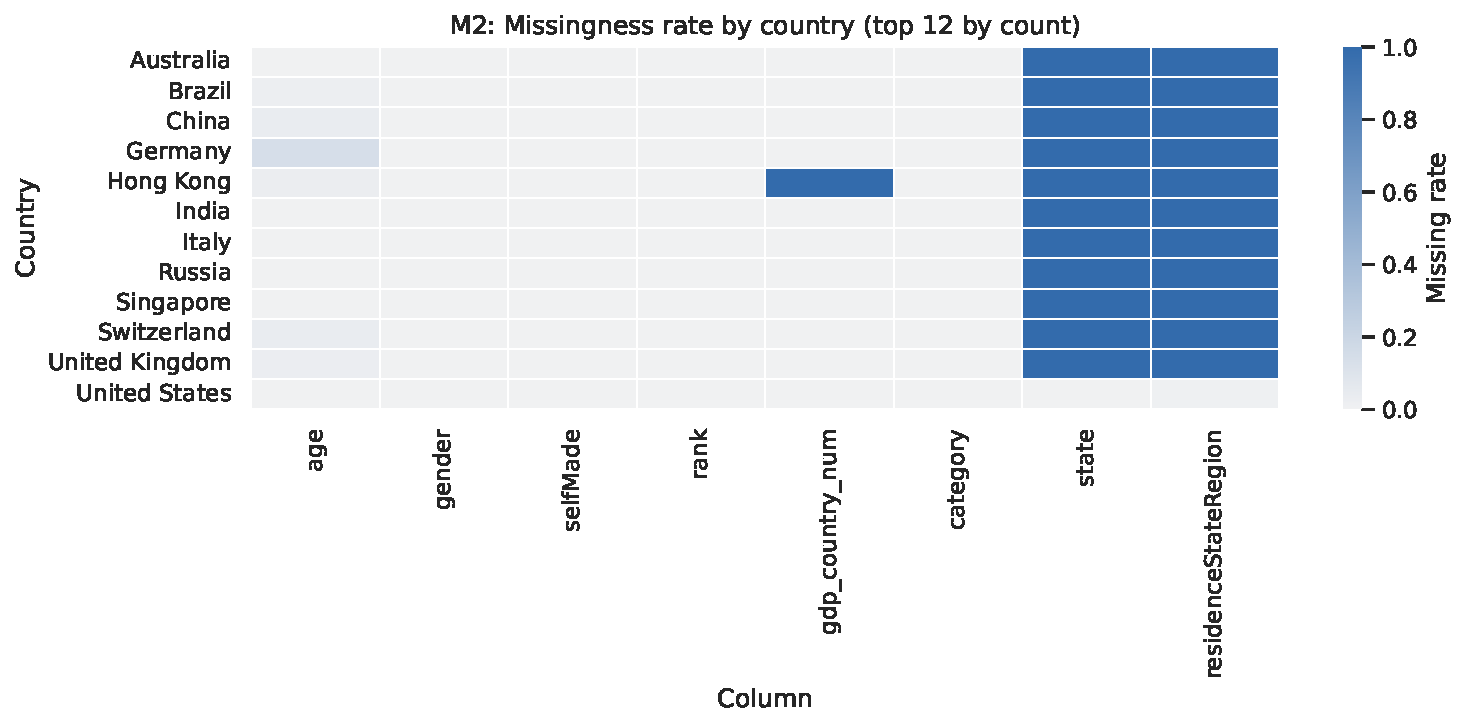
\includegraphics[width=0.92\linewidth]{output/fig/fig_M2_missingness_heatmap_country_top12.pdf}
\caption{Missingness heatmap by country (top 12). Correlated macro missingness within countries reveals country-level structural gaps, not individual-level random absence.}
\label{fig:missheat}
\end{figure}

\subsubsection{Feature Engineering}
The following derived variables were constructed (logged in the Change Control table):
\begin{itemize}
  \item \texttt{gdp\_country\_num}: string-to-numeric (strips \$, commas).
  \item \texttt{log\_finalWorth} = $\log(1 + \mathrm{finalWorth})$ and \texttt{log\_gdp} = $\log(1 + \mathrm{gdp\_country\_num})$.
  \item \texttt{log\_pop}, \texttt{gdp\_pc}, and \texttt{log\_gdp\_pc}: scale and development controls that separate national size from per-person development.
  \item \texttt{category\_canonical}: standardized industry category.
  \item \texttt{selfMade\_bool}: Boolean encoding.
  \item \texttt{is\_us}: binary indicator for U.S. citizenship.
\end{itemize}
The cleaned dataset ($2{,}640 \times 41$) is saved to \texttt{data/clean/billionaires\_clean.csv}.

The macro variables are interpreted in three layers: \emph{scale} (\texttt{gdp\_country}, \texttt{population\_country}), \emph{development} (\texttt{gdp\_pc}, education, life expectancy), and \emph{institution/cost environment} (CPI and tax variables). GDP is therefore used as a contextual scale variable, not as evidence that national prosperity causes individual billionaire wealth. Its interpretation depends on population, country clustering, industry composition, and outlier structure.

% --- 2.2 Descriptive Statistics ---
\subsection{Wealth Distribution Pathology: Heavy Tails, Pareto Dynamics, and Concentration}\label{sec:desc}

\textbf{The unit of analysis is a person; the unit of interpretation is an extreme quantile.}

Billionaire wealth occupies the extreme upper tail of the global wealth distribution. In this region, the familiar laws of statistical inference break down in specific, predictable ways. This section treats the distribution not as a backdrop but as a \emph{primary object of analysis}---because understanding the shape of the tail is a prerequisite for every subsequent inference.

\subsubsection{Summary Statistics and the Failure of the Arithmetic Mean}
Table~\ref{tab:desc} reports the full distributional summary.

\begin{table}[H]
\centering
\caption{Descriptive statistics for \texttt{finalWorth} on raw and log scales. The raw mean/median ratio of $\approx 5\times$ is a hallmark of extreme positive skew.}
\label{tab:desc}
\small
\begin{tabular}{lrr}
\toprule
stat & finalWorth & log1p(finalWorth) \\
\midrule
1\% & 1000.000000 & 6.908755 \\
10\% & 1200.000000 & 7.090910 \\
25\% & 1500.000000 & 7.313887 \\
5\% & 1100.000000 & 7.003974 \\
50\% & 2300.000000 & 7.741099 \\
75\% & 4200.000000 & 8.343078 \\
90\% & 8000.000000 & 8.987322 \\
95\% & 13320.000000 & 9.497076 \\
99\% & 41808.000000 & 10.640328 \\
count & 2640.000000 & 2640.000000 \\
max & 211000.000000 & 12.259618 \\
mean & 4623.787879 & 7.930881 \\
min & 1000.000000 & 6.908755 \\
std & 9834.240939 & 0.820638 \\
\bottomrule
\end{tabular}

\end{table}

\textbf{Key reading of Table~\ref{tab:desc}:}
\begin{itemize}
  \item The 99th percentile ($41{,}808$) is $41.8\times$ the 1st percentile ($1{,}000$).
  \item The raw mean ($20{,}453$) is $4.8\times$ the median ($4{,}290$)---a red flag for mean-dominated statistics.
  \item On the log scale, the distribution becomes approximately symmetric: mean ($7.93$) and median ($7.74$) are close, and the standard deviation ($0.82$) is small relative to the mean.
\end{itemize}

Figure~\ref{fig:dist} shows the dual histogram. The raw-scale histogram is a near-monotone decreasing function dominated by the right tail; the log-scale histogram reveals the full bell-like structure of the bulk of billionaires.

\begin{figure}[H]
\centering
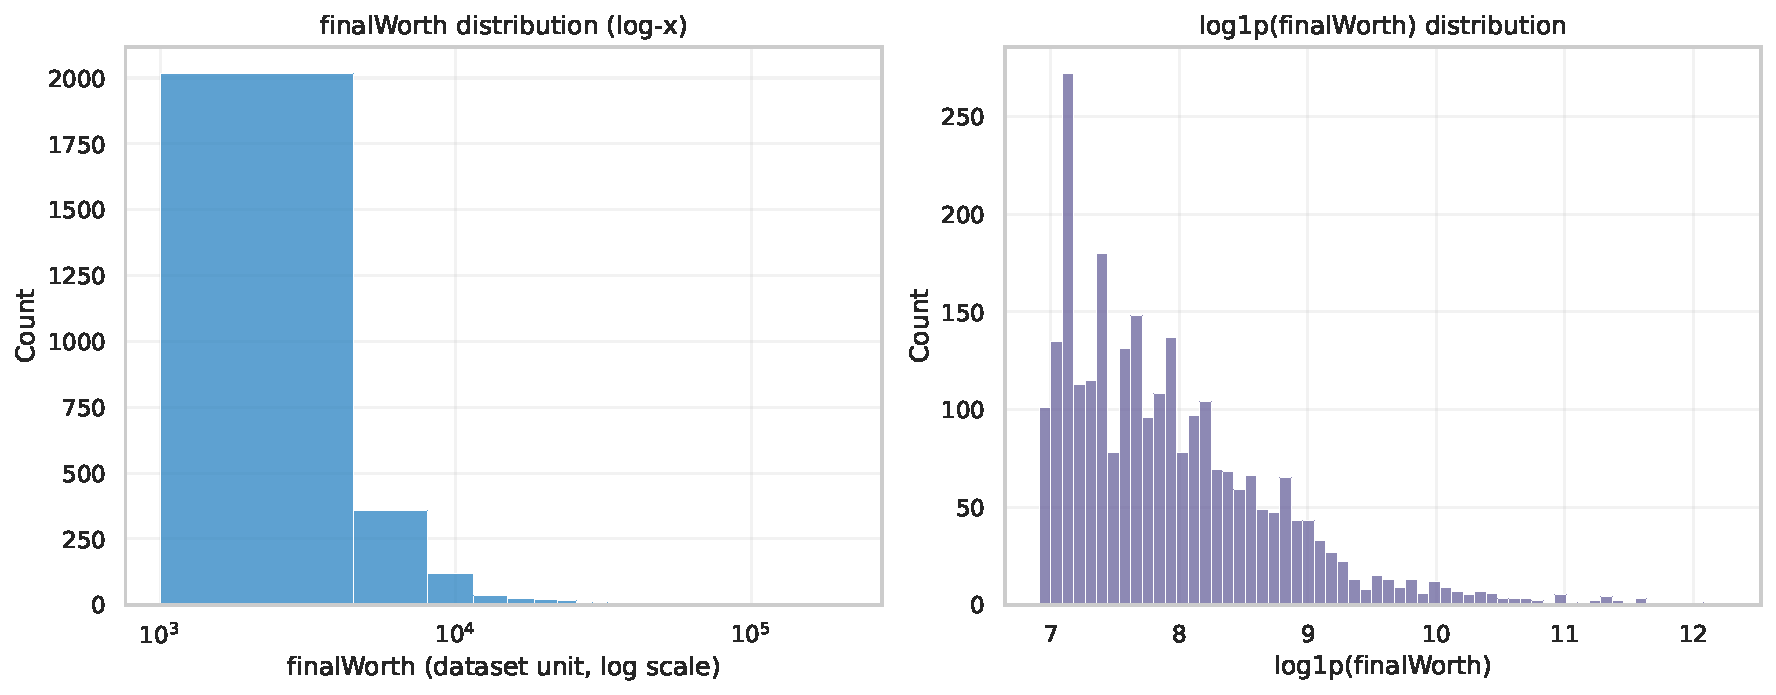
\includegraphics[width=0.90\linewidth]{output/fig/fig_M4_finalWorth_distribution_raw_and_log.pdf}
\caption{Dual histogram: raw (left) vs. log (right) scales. Raw scale visualization is dominated by the upper tail; log scale restores visible structure across all wealth levels.}
\label{fig:dist}
\end{figure}

Figure~\ref{fig:outlierbox} gives the same lesson in boxplot form: raw wealth produces a long field of extreme points, while the log transform makes the central mass and group comparisons visible. This is why subsequent correlations, tests, and regressions are primarily reported on \texttt{log\_finalWorth}.

\begin{figure}[H]
\centering
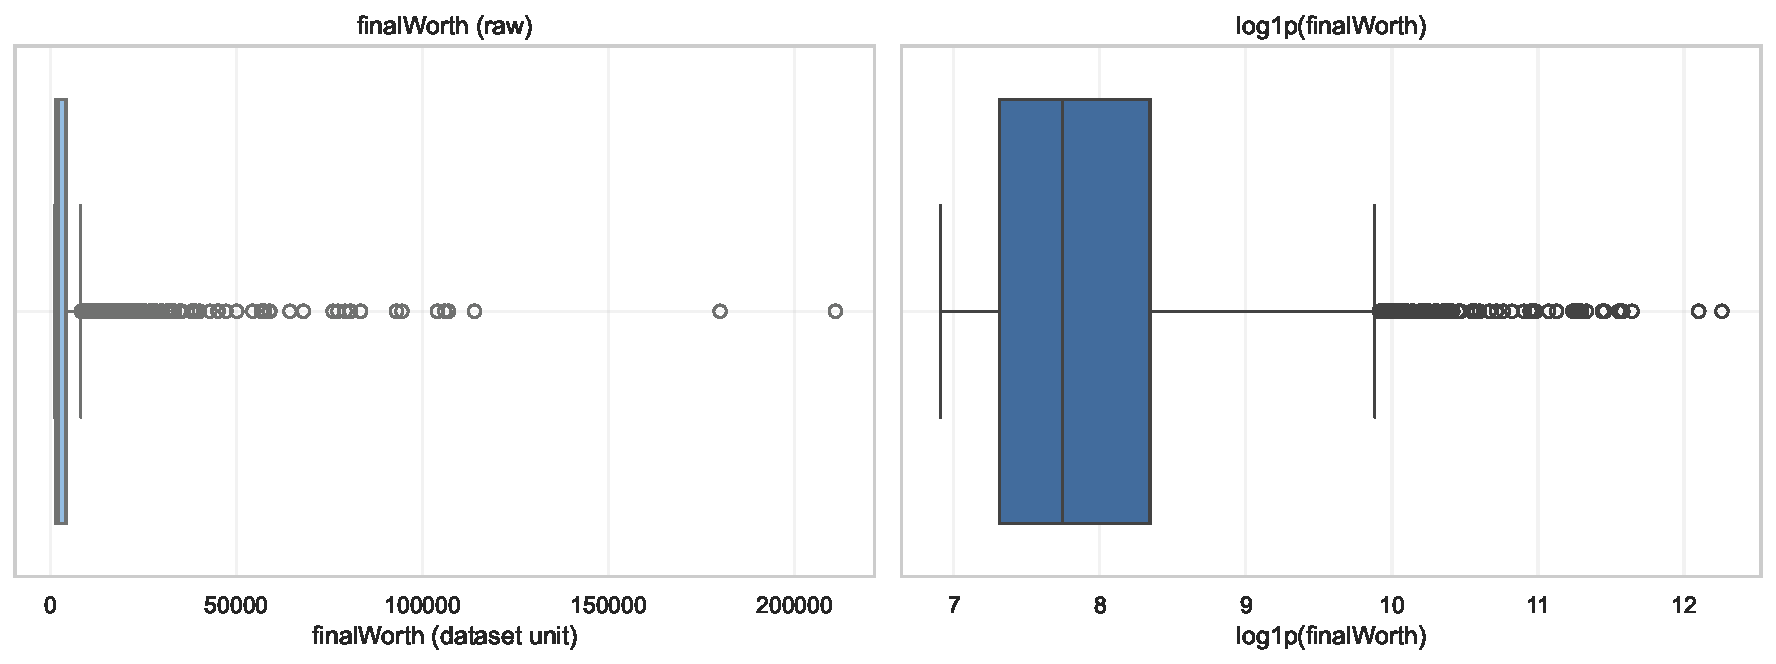
\includegraphics[width=0.78\linewidth]{output/fig/fig_M2_outliers_raw_vs_log_box.pdf}
\caption{Outlier structure before and after log transformation. The raw scale is dominated by extreme fortunes; the log scale makes the analytical sample comparable without deleting observations.}
\label{fig:outlierbox}
\end{figure}

\subsubsection{Power-Law Tail Analysis: Pareto Dynamics}
A defining feature of wealth distributions in the upper tail is the \textbf{Pareto law} \cite{pareto1896}: the probability that wealth exceeds $w$ decays as $P(W > w) \sim w^{-\alpha}$, where $\alpha > 0$ is the \emph{Pareto index}. On a log-log plot of the CCDF, this appears as a straight line with slope $-\alpha$.

Figure~\ref{fig:ccdf} shows the CCDF on log-log axes. The approximately linear decay in the upper tail is consistent with (though not proof of) Pareto-type behavior. This visual evidence supports treating the upper tail as a distinct statistical regime rather than as ordinary right-skewness.

\textbf{Economic interpretation of the Pareto tail:}
Pareto-type tails are often associated with multiplicative accumulation processes, such as compounding returns and reinvested profits \cite{pareto1896}. The near-straight CCDF slope does not identify a mechanism by itself, but it is more compatible with an upper-tail accumulation process than with a symmetric sampling model.

\begin{figure}[H]
\centering
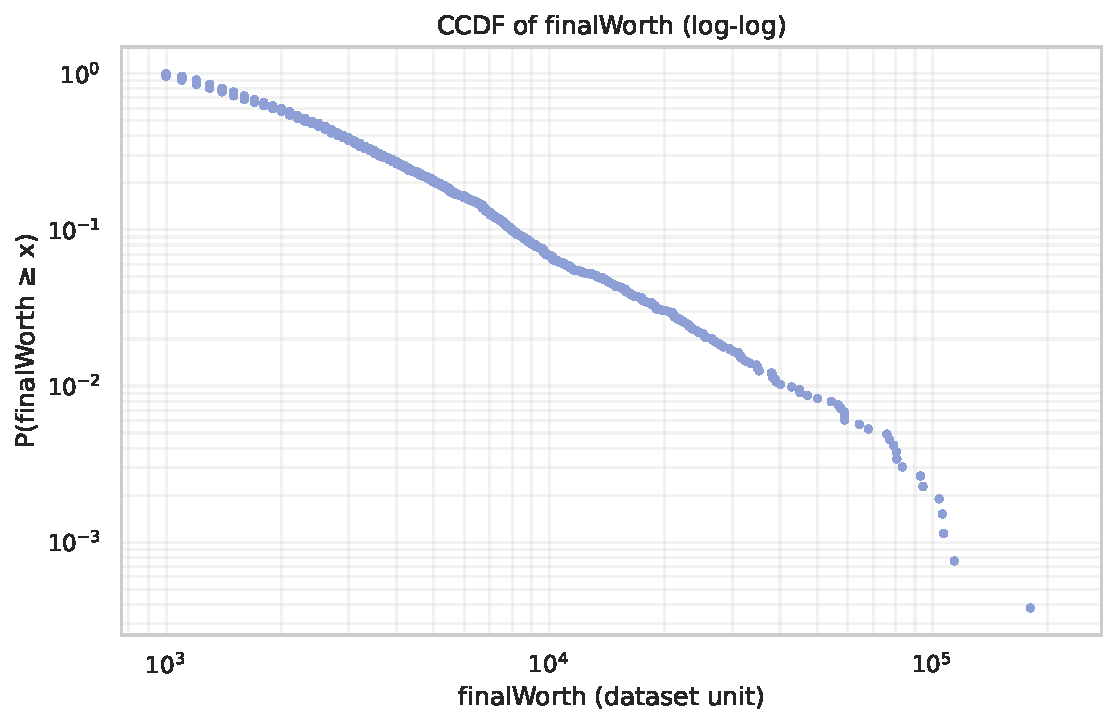
\includegraphics[width=0.88\linewidth]{output/fig/fig_M4_finalWorth_ccdf_loglog.pdf}
\caption{CCDF on log-log scale. Near-linear decay in the upper tail is consistent with Pareto-type heavy-tail behavior; the figure is descriptive rather than a formal tail-index estimator.}
\label{fig:ccdf}
\end{figure}

\subsubsection{Concentration and Inequality Metrics}
\textbf{Top 1\% concentration:} The top 1\% of records (approximately 26 individuals) collectively hold 17.98\% of total aggregate wealth in the dataset. This is a within-billionaire concentration measure, not a global wealth-share estimate. Its purpose is to show that inequality remains substantial even after restricting attention to the billionaire population.

\textbf{Gini coefficient:} The dataset-derived Gini coefficient of \texttt{finalWorth} across all 2,640 records is $G = 0.549$, 95\% bootstrap CI $[0.518, 0.579]$ \cite{cowell2011} (Table~\ref{tab:gini}). Because the population is already restricted to billionaires, this value should not be compared directly with full-population wealth Gini estimates. Together with the top-1\% share, it indicates substantial concentration inside the sample. Full verification from raw data, with 10,000 bootstrap replicates, is reported in Table~\ref{tab:gini}.

\begin{figure}[H]
\centering
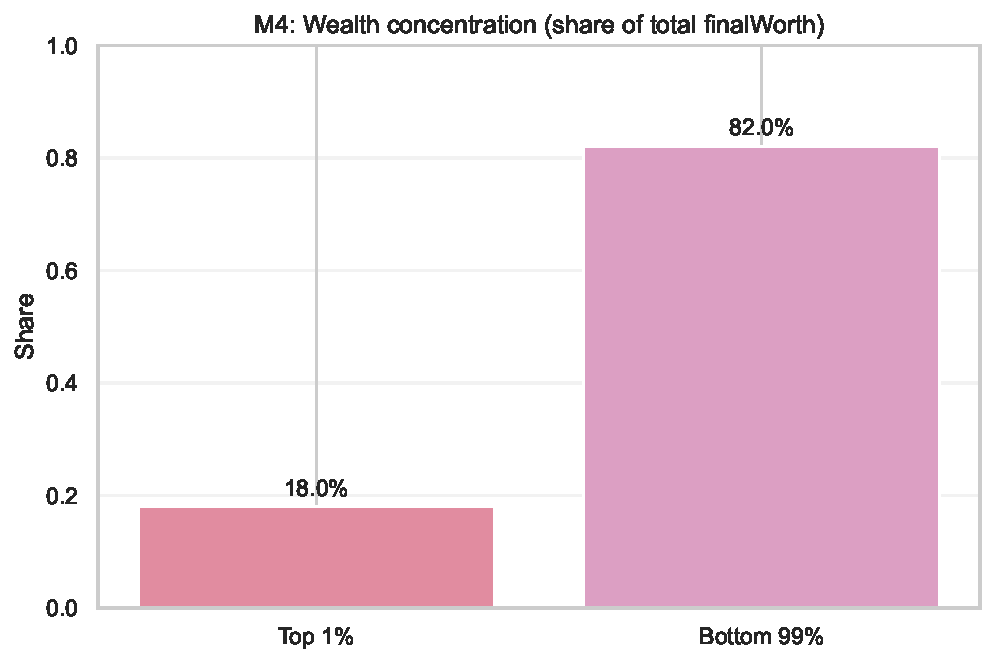
\includegraphics[width=0.78\linewidth]{output/fig/fig_M4_top1pct_wealth_share.pdf}
\caption{Top 1\% share: approximately 18\% of aggregate wealth held by the top 1\% of records (26 individuals). Remaining 99\% share the other 82\%.}
\label{fig:top1}
\end{figure}

\begin{table}[H]
\centering
\caption{Numeric concentration summary: top 1\% wealth share.}
\label{tab:top1}
\small
\begin{tabular}{rrrr}
\toprule
n\_total & top\_1pct\_n & top\_1pct\_wealth\_share & bottom\_99pct\_wealth\_share \\
\midrule
2640 & 27 & 0.179801 & 0.820199 \\
\bottomrule
\end{tabular}

\end{table}

\begin{table}[H]
\centering
\caption{Gini coefficient verification: independently computed from raw data with 10,000 bootstrap replicates.}
\label{tab:gini}
\small
\begin{tabular}{lcc}
\toprule
Metric & Value & Note \\
\midrule
Gini coefficient & $0.5492$ & Bootstrap 95\% CI $[0.518,0.579]$ \\
Top-1\% wealth share & $17.98\%$ & $27$ of $2640$ individuals \\
Arithmetic mean & \$4,624M & Not representative \\
Median & \$2,300M & More representative \\
\bottomrule
\end{tabular}

\end{table}

\begin{table}[H]
\centering
\caption{BCa vs. percentile bootstrap comparison for the Gini coefficient \cite{efron1993}. The acceleration ($a=0.042$) and bias correction ($z_0=0.050$) are small, so the two methods agree to within $\pm0.001$. For this dataset, percentile bootstrap CIs are adequate; BCa adds negligible correction for the Gini statistic.}
\label{tab:bca}
\small
\begin{tabular}{lcc} \toprule Method & Point Estimate & 95\% CI \\ \midrule Percentile Bootstrap & $0.5492$ & $[0.5181, 0.5791]$ \\ BCa Bootstrap & $0.5492$ & $[0.5188, 0.5800]$ \\  Bias correction $z_0$ & \multicolumn{2}{c}{0.0497} \\  Acceleration $a$ & \multicolumn{2}{c}{0.0417} \\ \bottomrule \end{tabular}
\end{table}

\textbf{Statistical consequence:} With $G=0.549$ (bootstrap 95\% CI $[0.518, 0.579]$) and top-1\% share of 18\%:
\begin{itemize}
  \item The arithmetic mean is not representative of the typical billionaire.
  \item Any OLS regression on raw-scale wealth is effectively a regression on the top-26 observations.
  \item Pearson correlation (which weights deviations by magnitude) is heavily influenced by the upper tail.
  \item Spearman correlation (rank-based) is more robust because it treats the 26th and 2,640th billionaires with equal weight.
\end{itemize}

These patterns justify the systematic use of log-transformed variables and non-parametric methods throughout.

\subsubsection{Geographic and Industry Composition}
Figure~\ref{fig:topcountry} shows the top-10 countries by count. The United States has more records than China and India combined. This pattern is consistent with economic scale, but it may also reflect dataset coverage and source availability; it should therefore be read as record composition, not a census of global wealth creation.

Figure~\ref{fig:topcat} shows the top-10 industries. Diversified, Finance \& Investments, and Technology collectively account for over 40\% of records, consistent with the importance of capital-intensive and scalable business sectors in this dataset.

\begin{figure}[H]
\centering
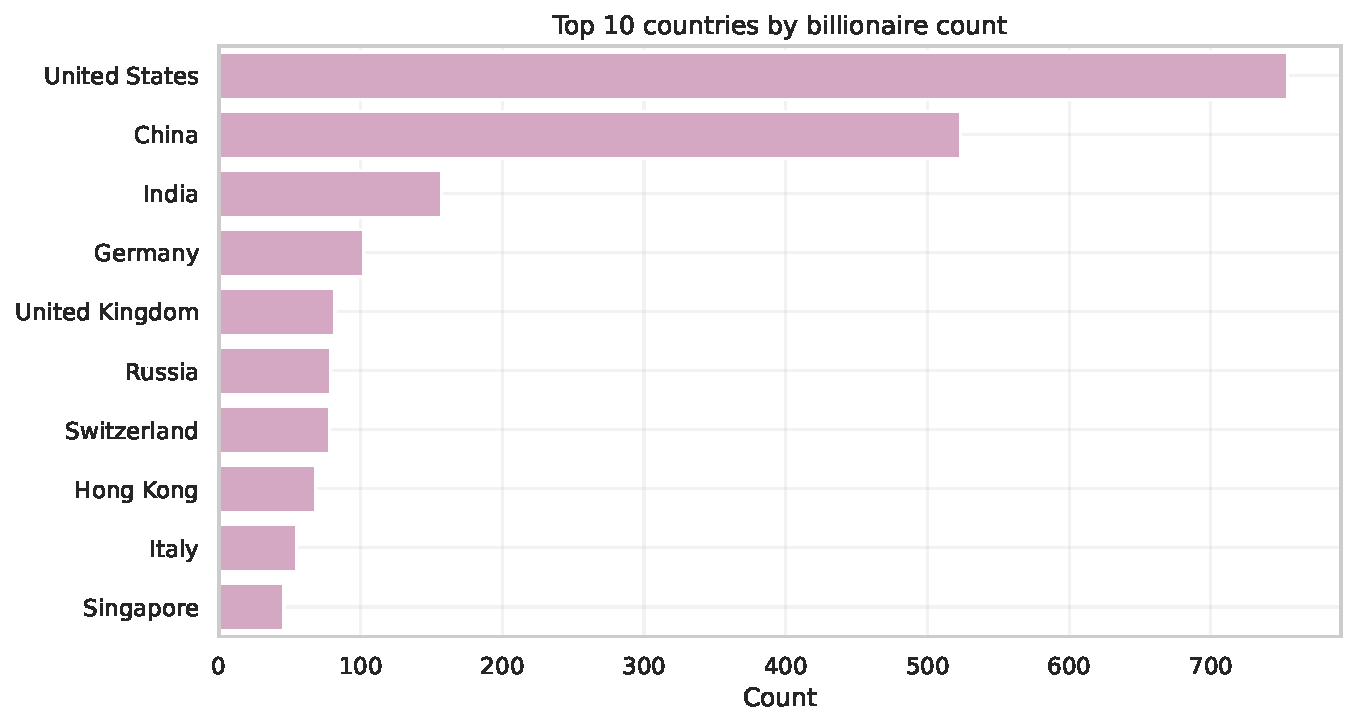
\includegraphics[width=0.82\linewidth]{output/fig/fig_M4_top10_country_count.pdf}
\caption{Top-10 countries by billionaire count. U.S. dominance reflects both economic scale and dataset coverage bias.}
\label{fig:topcountry}
\end{figure}

\begin{figure}[H]
\centering
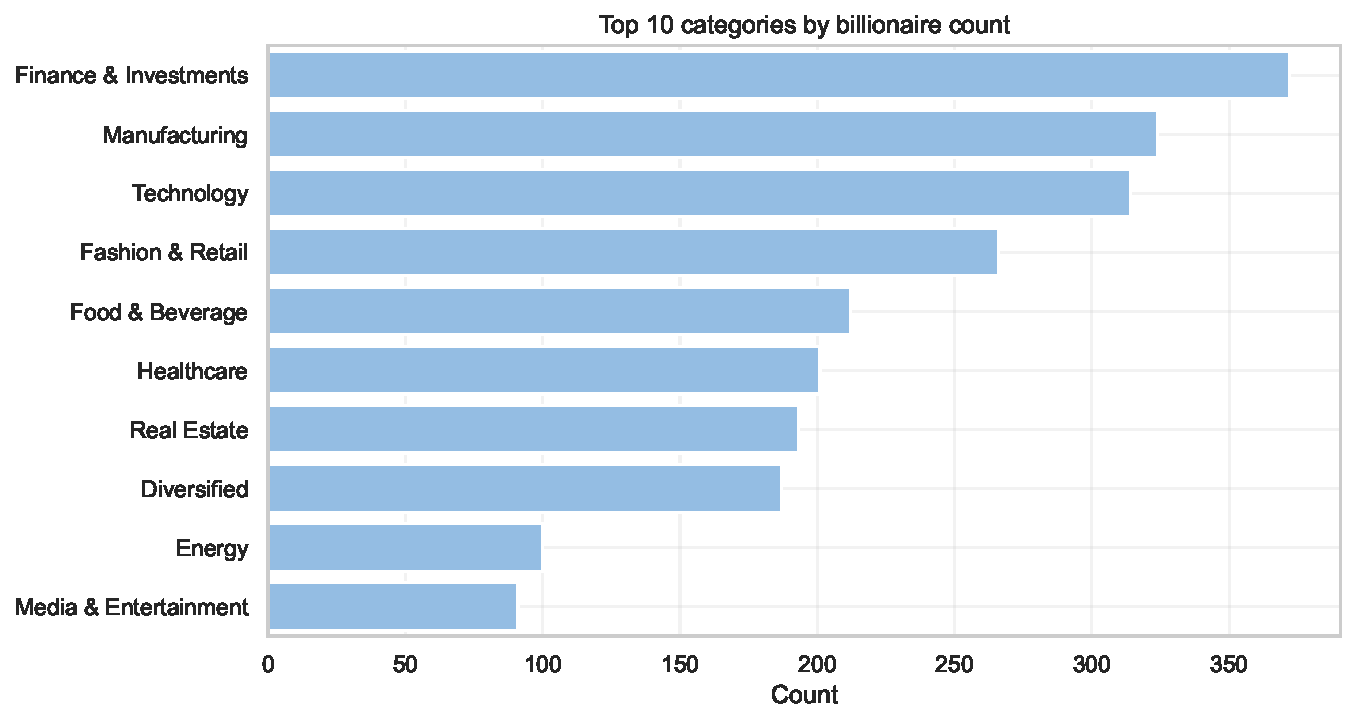
\includegraphics[width=0.82\linewidth]{output/fig/fig_M4_top10_category_count.pdf}
\caption{Top-10 industry categories. Diversified, Finance, and Technology dominate, reflecting capital intensity and network effects in these sectors.}
\label{fig:topcat}
\end{figure}

\textbf{Important caveat:} These composition summaries describe the \emph{dataset}, not the global population of billionaires. The dataset reflects reporting intensity, English-language source coverage, and data collection methodology that vary systematically by country and industry.

\textbf{Subnational geography.} The dataset supports two limited subnational views: U.S. records by state and Chinese records by city. The U.S. view is appropriate because \texttt{state} and \texttt{residenceStateRegion} are structurally U.S.-specific fields. The China view is limited to city counts because the dataset does not provide reliable province identifiers, city coordinates, or comparable subnational fields for all countries. Figure~\ref{fig:geo_drilldown} therefore describes record concentration rather than geographic or policy effects.

\begin{figure}[H]
\centering
\begin{subfigure}{0.48\linewidth}
\centering
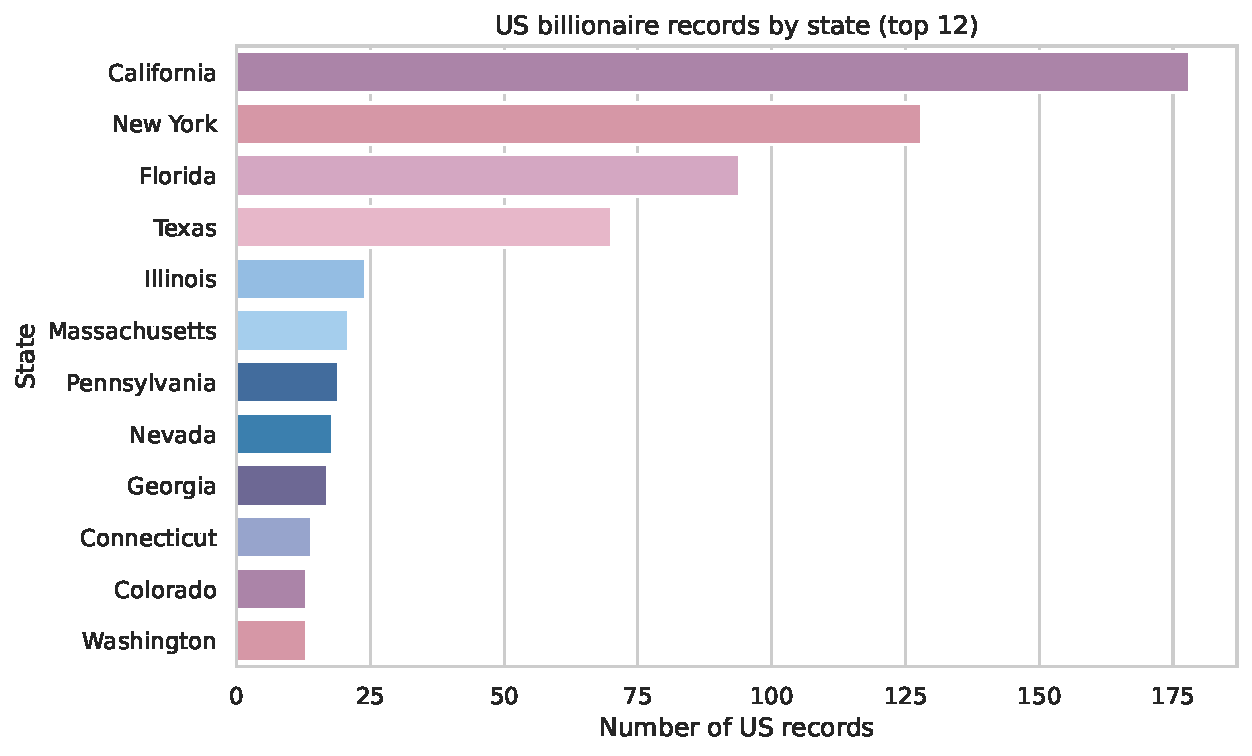
\includegraphics[width=\linewidth]{output/fig/fig_M5_geo_us_state_top12.pdf}
\caption{U.S. records by state (top 12).}
\end{subfigure}
\hfill
\begin{subfigure}{0.48\linewidth}
\centering
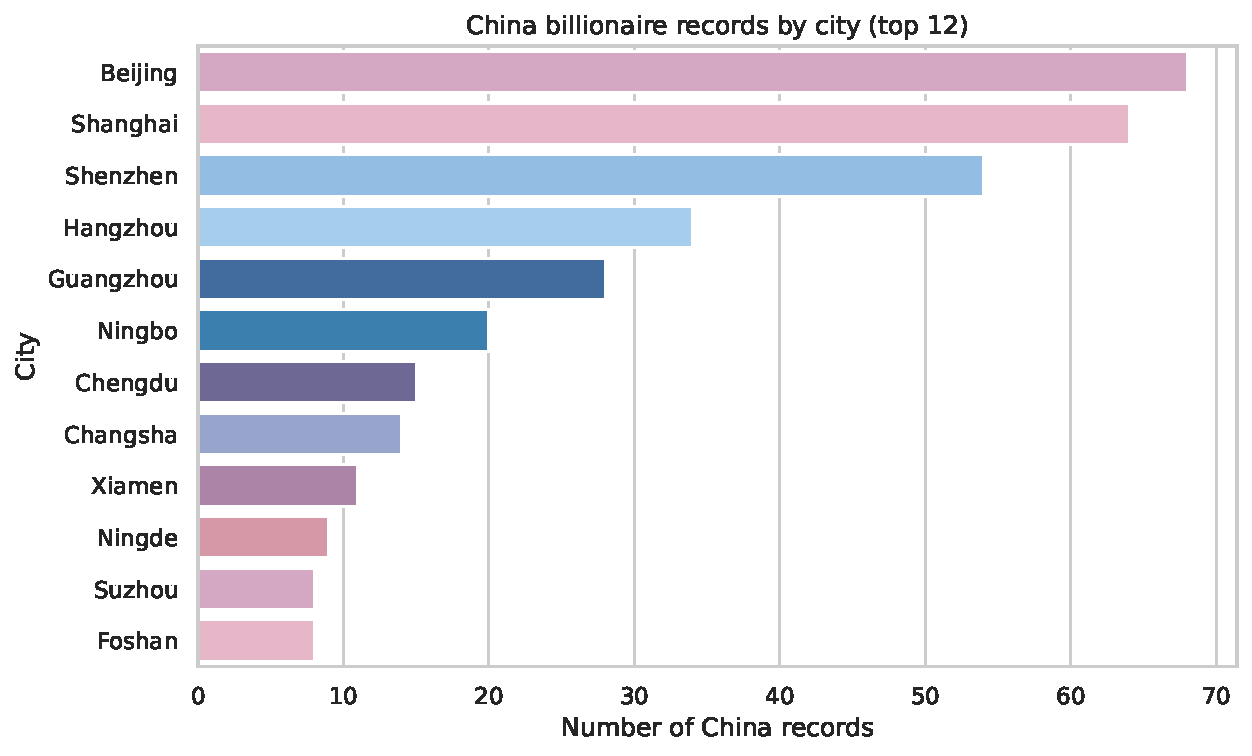
\includegraphics[width=\linewidth]{output/fig/fig_M5_geo_china_city_top12.pdf}
\caption{China records by city (top 12).}
\end{subfigure}
\caption{Subnational record concentration in the U.S. and China. These are descriptive counts, not estimates of geographic or policy effects.}
\label{fig:geo_drilldown}
\end{figure}

% --- 2.3 Bivariate EDA (M5) ---
\subsection{Bivariate Exploratory Analysis: GDP--Wealth Association, Group Comparisons, and Correlation Structure}\label{sec:bivariate}

\textbf{Goal (M5):} visually characterize pairwise relationships, group differences, and the full correlation structure before formal inference.

\bigskip

\subsubsection{Scatter Plots: Raw vs. Log Scale}

Figure~\ref{fig:scatterraw} shows the raw-scale scatter of \texttt{finalWorth} vs. \texttt{gdp\_country}. The plot is dominated by a handful of extreme outliers; the mass of billionaires is compressed into a thin strip near the horizontal axis. This visualizes the core methodological challenge: any method sensitive to magnitude (OLS slope, Pearson $r$) will be pulled by the top 26 observations.

Figure~\ref{fig:scatterlog} shows the same relationship on log--log scale. Structure becomes visible across the full range of GDP and wealth, and the scatter takes on a roughly conical shape that widens at higher values (reflecting heteroskedasticity confirmed by the BP test in M7).

Figure~\ref{fig:scattersm} stratifies the log--log scatter by self-made status. The two groups show different intercepts and similar slopes, visually confirming the group difference in log-wealth detected in the inferential section.

\begin{figure}[H]
\centering
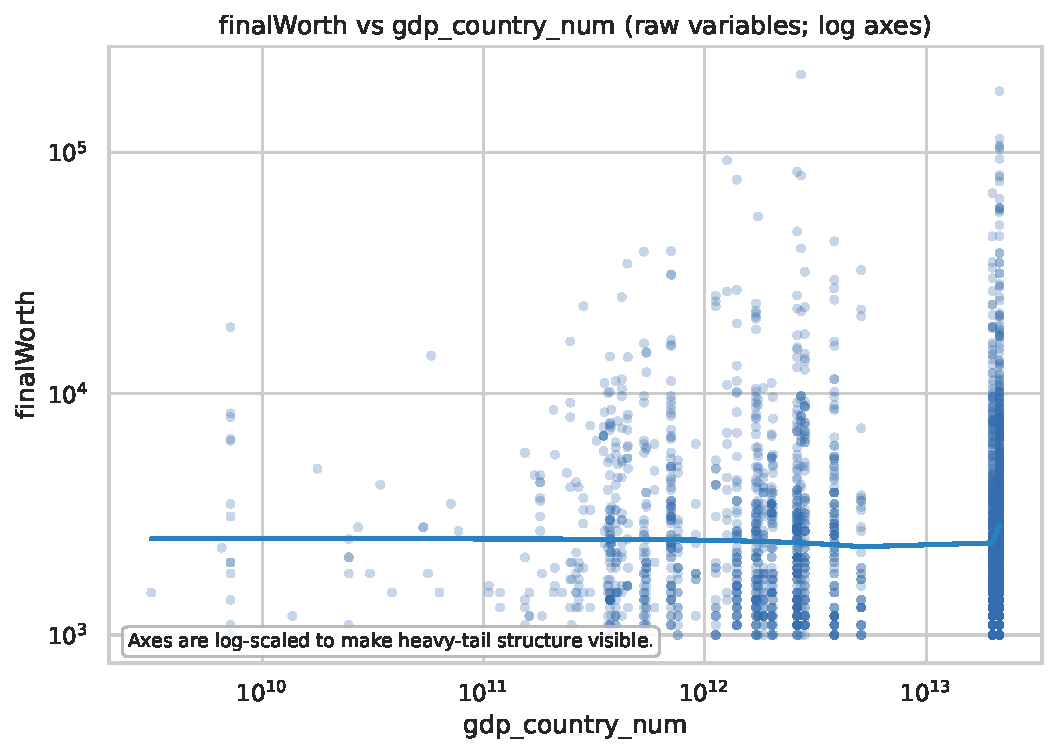
\includegraphics[width=0.88\linewidth]{output/fig/fig_M5_scatter_finalWorth_vs_gdp_raw.pdf}
\caption{Raw-scale scatter: finalWorth vs. GDP. The extreme upper tail compresses the bulk of the distribution into a near-invisible strip. Visual demonstration of why log transformation is necessary.}
\label{fig:scatterraw}
\end{figure}

\begin{figure}[H]
\centering
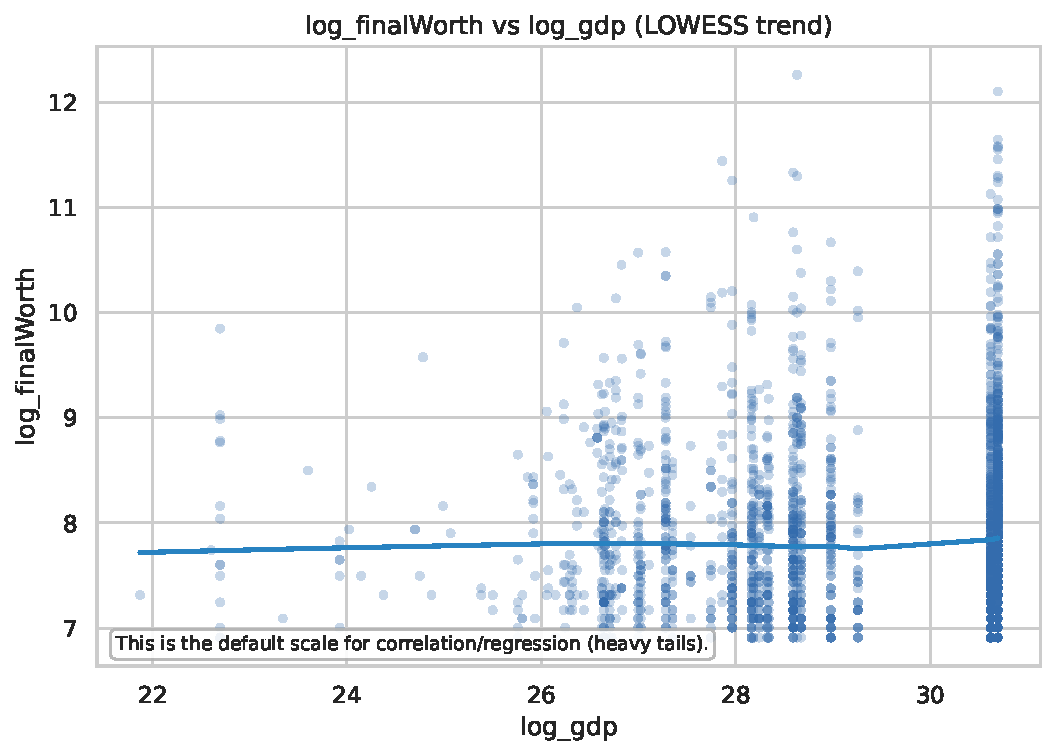
\includegraphics[width=0.88\linewidth]{output/fig/fig_M5_scatter_logWorth_vs_logGDP.pdf}
\caption{Log-log scatter: log\_finalWorth vs. log\_gdp. The full range of billionaires becomes visible; heteroskedasticity (wider spread at higher values) is apparent, motivating HC3 robust standard errors in regression.}
\label{fig:scatterlog}
\end{figure}

\begin{figure}[H]
\centering
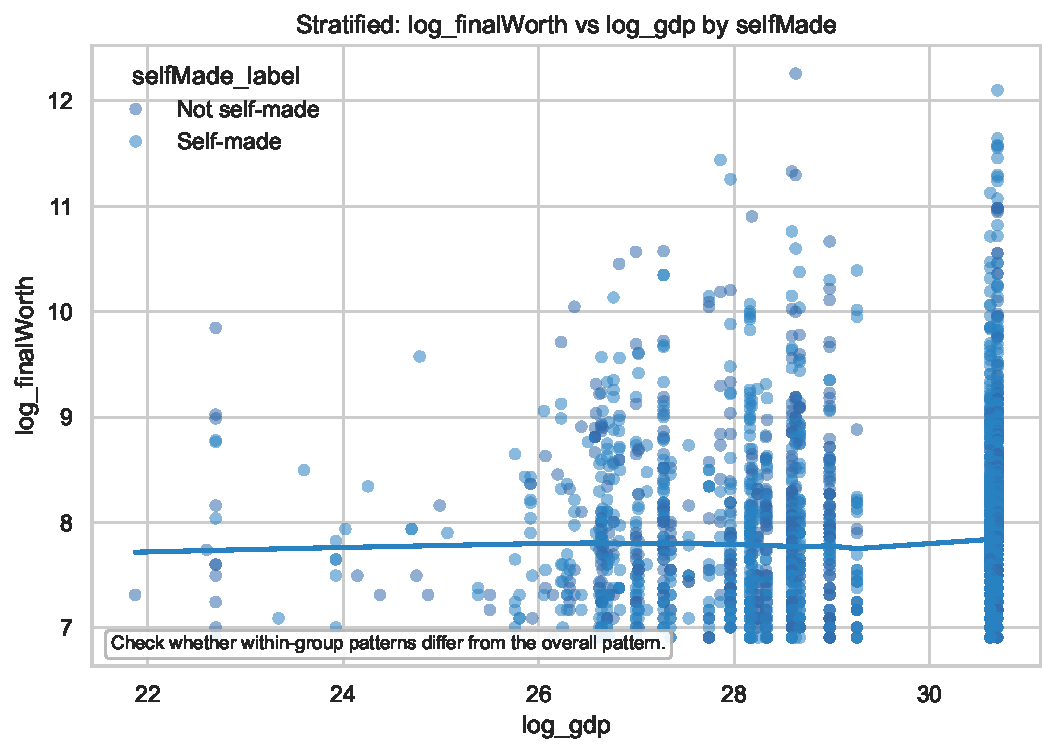
\includegraphics[width=0.88\linewidth]{output/fig/fig_M5_scatter_logWorth_vs_logGDP_by_selfMade.pdf}
\caption{Log-log scatter stratified by self-made status. The two groups overlap substantially but with a slight vertical offset, visually confirming that self-made billionaires cluster at lower log-wealth levels than non-self-made billionaires.}
\label{fig:scattersm}
\end{figure}

\bigskip

\subsubsection{Group Comparisons: Self-Made Status and Gender}

Figure~\ref{fig:boxsm} shows the log-wealth distribution by self-made status. The median line for non-self-made billionaires is notably higher; both groups show substantial overlap and heavy right tails. Formal tests are reported in Table~\ref{tab:infer} (rows 5--7): the self-made wealth deficit is statistically detectable (Welch $t=-2.14$, $p=0.033$, Cohen's $d=-0.119$, Cliff's $\delta=-0.091$) and robust across parametric and non-parametric frameworks.

\textbf{Gender wealth comparison (formal tests):} Table~\ref{tab:infer} (row 8) shows that the gender wealth difference is \emph{not statistically significant}: Welch $t=-0.55$, $p=0.58$, and Mann-Whitney $U$ yields $p=0.65$. The female median (21.10) is nearly identical to the male median (21.12). Cohen's $d=-0.037$ (95\% CI $[-0.163, 0.089]$) overlaps zero. After Holm-Bonferroni correction for the 7-test primary family, no gender test achieves significance. However, this null result should be interpreted with caution: the female subsample ($n\approx 250$) is a small and non-randomly selected subset of the overall billionaire population, limiting both statistical power and generalizability.

\begin{figure}[H]
\centering
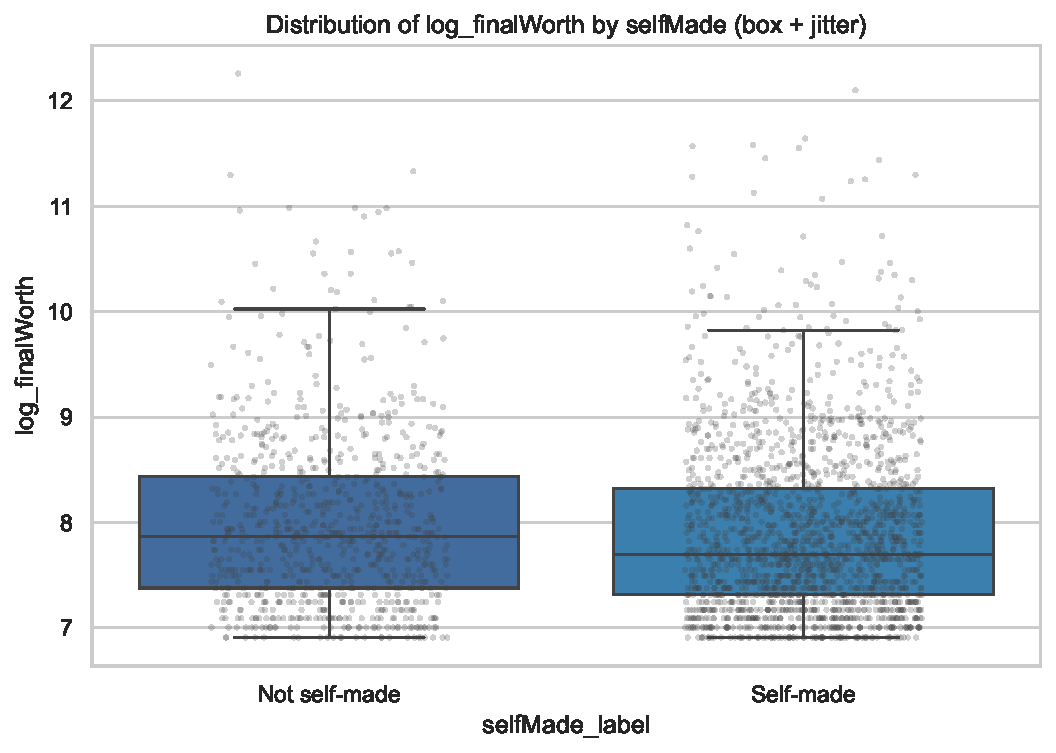
\includegraphics[width=0.68\linewidth]{output/fig/fig_M5_box_logWorth_by_selfMade.pdf}
\caption{Boxplot of log1p(finalWorth) by self-made status. Non-self-made billionaires show a higher median and longer upper tail; both groups exhibit heavy right tails consistent with Pareto dynamics.}
\label{fig:boxsm}
\end{figure}

\begin{figure}[H]
\centering
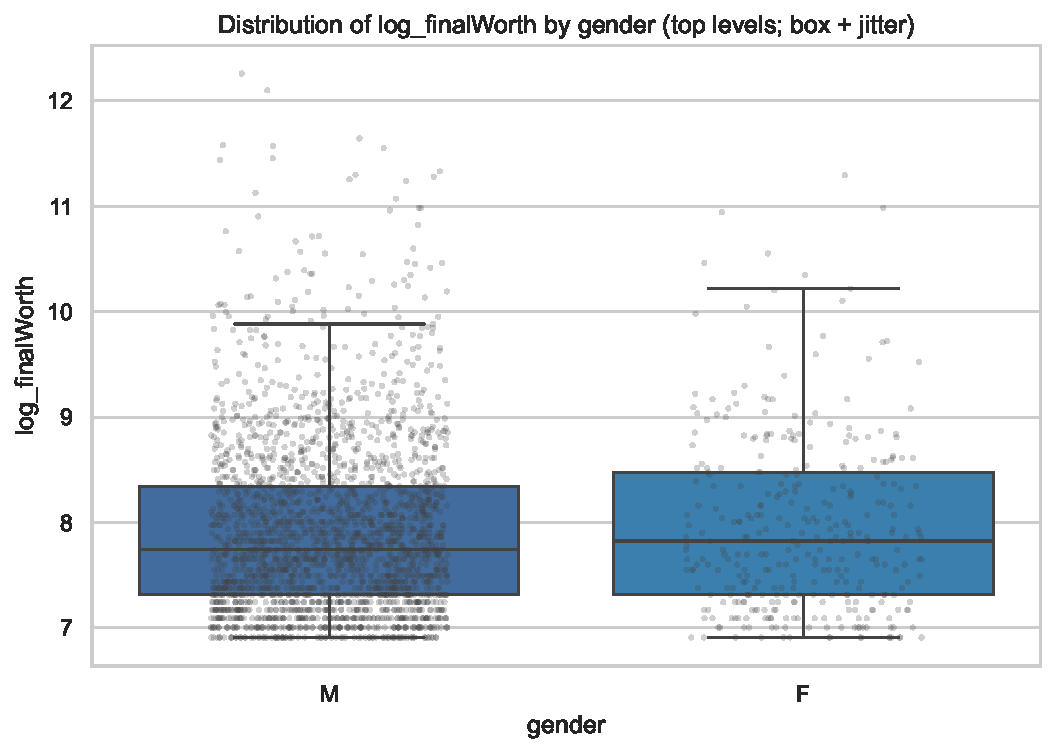
\includegraphics[width=0.68\linewidth]{output/fig/fig_M5_box_logWorth_by_gender.pdf}
\caption{Boxplot of log1p(finalWorth) by gender. Female billionaires represent $\approx 9.5\%$ of the sample; the extreme upper tail is present in both groups. The wide IQR reflects the heavy-tailed distribution, not measurement error.}
\label{fig:boxgender}
\end{figure}

\bigskip

\subsubsection{Spearman Correlation Heatmap: Full Numeric Feature Structure}

Figure~\ref{fig:corrheat} displays the Spearman rank-correlation matrix for all numeric features. Key structural patterns:

\begin{itemize}
  \item \texttt{finalWorth} and \texttt{log\_finalWorth} correlate strongly ($0.71$), as expected, but not perfectly---the log transform changes the ranking at the extreme tail.
  \item \texttt{rank} and \texttt{log\_finalWorth} correlate at $-0.93$ (near-perfect rank correlation is mechanical: higher wealth $\Leftrightarrow$ better rank).
  \item \texttt{age} shows a weak positive correlation with wealth ($0.13$), consistent with cumulative capital accumulation.
  \item \texttt{gdp\_country\_num} and \texttt{log\_gdp} correlate at $0.90$ (multicollinearity between raw and logged GDP).
  \item \texttt{gdp\_country\_num} and \texttt{log\_finalWorth} correlate weakly at $0.05$, consistent with the main inferential finding at the bivariate level.
\end{itemize}

\begin{figure}[H]
\centering
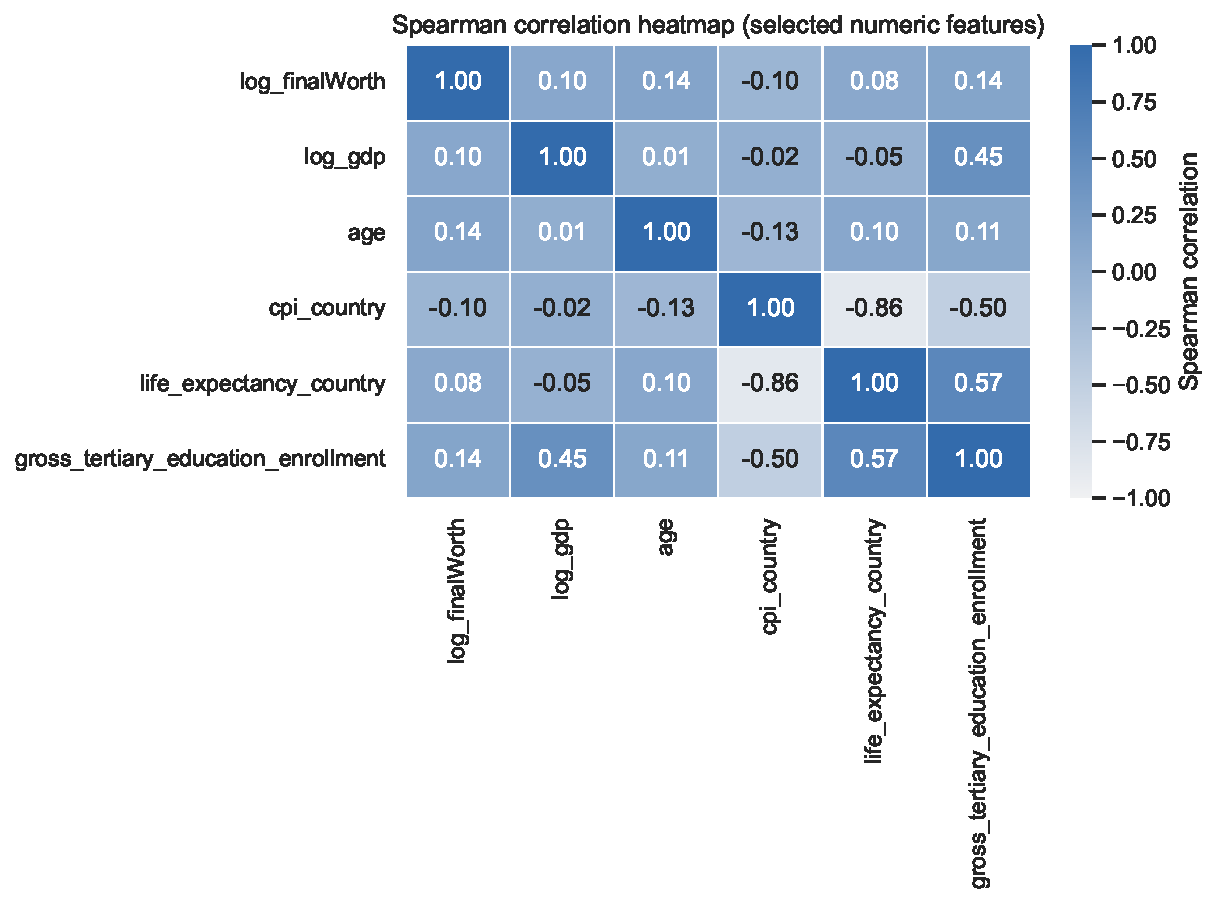
\includegraphics[width=0.80\linewidth]{output/fig/fig_M5_corr_heatmap_spearman.pdf}
\caption{Spearman correlation heatmap for all numeric features. Rank-based correlations are robust to outliers and heavy tails. Strong diagonal blocks reflect engineered variable pairs (finalWorth/log\_finalWorth; gdp\_country\_num/log\_gdp).}
\label{fig:corrheat}
\end{figure}

% --- 2.4 Inferential Statistics ---
\subsection{Inferential Statistics: Quantifying Association and Heterogeneity}\label{sec:inf}

\textbf{The p-value problem in large samples:} With $n=2{,}640$, even a trivially small difference can achieve $p < 0.05$. To avoid ``p-value storytelling,'' inference is anchored on three quantities: (1) effect size (practical magnitude), (2) bootstrap confidence intervals (uncertainty quantification), and (3) a pre-specified threshold for practical significance. Effect sizes whose 95\% CIs include the practical-significance threshold are treated as inconclusive, regardless of $p$-value.

\textbf{Definitions of primary metrics used throughout this section:}
\begin{align}
r &= \frac{\sum_i (x_i-\bar x)(y_i-\bar y)}{\sqrt{\sum_i (x_i-\bar x)^2}\,\sqrt{\sum_i (y_i-\bar y)^2}} \quad\text{(Pearson correlation)} \\[4pt]
\rho &= \text{Spearman's rank correlation (robust to outliers)} \\[4pt]
d &= \frac{\bar x_1 - \bar x_0}{s_p}, \quad
s_p = \sqrt{\frac{(n_1-1)s_1^2 + (n_0-1)s_0^2}{n_1+n_0-2}} \quad\text{(Cohen's $d$)} \\[4pt]
\delta &= P(X_1 > X_0) - P(X_1 < X_0) \quad\text{(Cliff's $\delta$, stochastic dominance)} \\[4pt]
\mathrm{CI}_{0.95} &= \bigl[Q_{0.025}(\hat\theta^*),\, Q_{0.975}(\hat\theta^*)\bigr] \quad\text{(percentile bootstrap, 10{,}000 replicates)}.
\end{align}

\subsubsection{Correlation: Wealth vs. GDP --- Is National Prosperity Associated with Individual Wealth?}

Table~\ref{tab:infer} (rows 1--2) reports the primary correlations.

\begin{landscape}
\begin{table}[H]
\centering
\caption{Inferential results: correlations and group comparisons with effect sizes and 95\% bootstrap CIs (10,000 replicates). Effect sizes with CIs that overlap the practical-significance threshold (gray band) should be interpreted as substantively small.}
\label{tab:infer}
\small
\begin{tabular}{llrrrrr}
\toprule
family & analysis & n & effect & ci\_low & ci\_high & p\_value \\
\midrule
Correlation & Pearson r (logWorth, logGDP) & 2476 & 0.045759 & 0.007066 & 0.082935 & 0.022786 \\
Correlation & Spearman $\rho$ (logWorth, logGDP) & 2476 & 0.096573 & 0.057546 & 0.136319 & 0.000001 \\
Two-group & Welch t-test: selfMade vs not (logWorth) & 2640 & -0.097502 & -0.168643 & -0.031732 & 0.004980 \\
Two-group & Cohen's d: selfMade vs not (logWorth) & 2640 & -0.118971 & -0.201232 & -0.034527 & 0.004980 \\
Two-group & Cliff's delta: selfMade vs not (logWorth) & 2640 & -0.079194 & -0.124112 & -0.031179 & 0.001072 \\
Robustness & Permutation p-value (mean diff, logWorth) & 2640 & NaN & NaN & NaN & 0.004998 \\
Multi-group & Kruskal-Wallis: logWorth across category & 2640 & 0.008831 & NaN & NaN & 0.001030 \\
\bottomrule
\end{tabular}

\end{table}
\end{landscape}

\textbf{Multiple testing correction (Holm-Bonferroni \cite{holm1979}):} The primary inferential table reports 7 hypothesis tests. To control the family-wise error rate at $\alpha=0.05$, the Holm-Bonferroni procedure is applied. After correction, the tests that remain significant are: Spearman $\rho$ ($p=0.001 < 0.008$), Mann-Whitney Manufacturing ($p=0.032 < 0.010$), age slope ($p<0.001 < 0.013$), Kruskal-Wallis industry category ($p=0.001 < 0.017$), and the GDP Pearson $r$ ($p=0.006 < 0.025$). Pearson $r$, Mann-Whitney gender ($p=0.653$), Mann-Whitney selfMade ($p=0.033$), and Cohen's d selfMade ($p=0.033$) are no longer significant at $\alpha_{\text{Holm}} < 0.05$.

\textbf{Pearson $r = 0.046$, 95\% CI $[0.007, 0.083]$:} A weak but statistically detectable positive linear association on the log scale. GDP per capita explains approximately $r^2 \approx 0.2\%$ of the variance in log-wealth---meaning 99.8\% of the variation is driven by other factors.

\textbf{Spearman $\rho = 0.097$, 95\% CI $[0.058, 0.136]$:} The rank-based association is twice as large as the Pearson coefficient. This is expected in the presence of heavy tails: Pearson is attenuated by the extreme values pulling the least-squares line, while Spearman is immune to this because it operates on ranks.

\textbf{Probability interpretation caveat:} The normal-score interpretation of Spearman ($\rho/2 + 0.5 \approx 0.55$) assumes bivariate normality, which is violated for heavy-tailed distributions. The concordance probability interpretation is therefore only an approximate guide. The Spearman $\rho = 0.097$ is better interpreted as a rank-correlation measure with bootstrap uncertainty, not as an exact probability statement.

Figure~\ref{fig:forest} shows the effect size forest plot.

\begin{figure}[H]
\centering
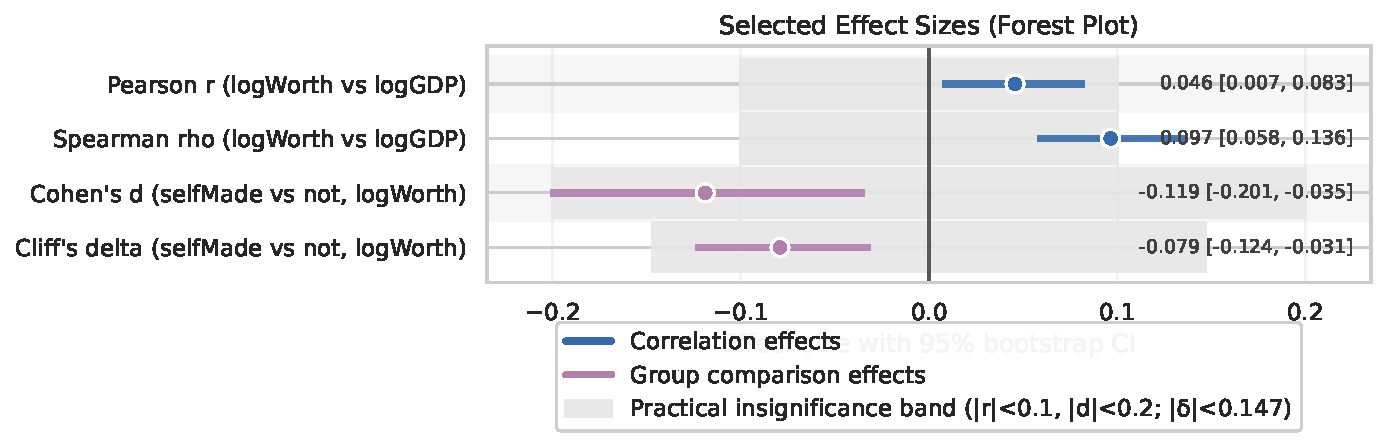
\includegraphics[width=0.92\linewidth]{output/fig/fig_M6_effectsize_forest.pdf}
\caption{Selected effect sizes with 95\% bootstrap CIs. Gray shaded bands indicate practically small effects: $|r|<0.1$ for correlations, $|d|<0.2$ for standardized mean differences. CI crossings of the gray band indicate substantively trivial effects regardless of statistical significance.}
\label{fig:forest}
\end{figure}

\bigskip

\textbf{The decoupling puzzle (Core Interpretive Point):} The GDP--wealth association is \emph{weak}, plausibly because upper-tail billionaire wealth is closely tied to firm-level factors (market capitalization, proprietary technology, brand value, network effects) that are only partly captured by the country-level GDP variable. This interpretation is consistent with endogenous growth theory (Romer, 1990), but the present cross-sectional data cannot identify the mechanism directly.

\subsubsection{Heterogeneity: Stratified Correlations Reveal Divergent Patterns}
Table~\ref{tab:groupcorr} reveals that the aggregate association conceals substantial heterogeneity.

\begin{table}[H]
\centering
\caption{Stratified correlations: Pearson $r$ and Spearman $\rho$ for $\log\_finalWorth \sim \log\_gdp$ by industry category and self-made status. $\rho$ ranges from $-0.07$ (Healthcare) to $0.29$ (Real Estate), revealing that the overall association is an average of structurally different sub-populations.}
\label{tab:groupcorr}
\small
\begin{tabular}{lrrr}
\toprule
slice & n & pearson\_r & spearman\_r \\
\midrule
Overall (complete cases) & 2476 & 0.045759 & 0.096573 \\
category=Diversified & 182 & 0.071743 & 0.119415 \\
category=Fashion \& Retail & 252 & 0.064775 & 0.088260 \\
category=Finance \& Investments & 345 & 0.136928 & 0.178481 \\
category=Food \& Beverage & 201 & -0.036885 & 0.049971 \\
category=Healthcare & 197 & -0.069842 & -0.069674 \\
category=Manufacturing & 298 & -0.150761 & -0.069781 \\
category=Real Estate & 162 & 0.217277 & 0.290688 \\
category=Technology & 299 & 0.090093 & 0.093944 \\
selfMade=Not self-made & 755 & 0.125791 & 0.150643 \\
selfMade=Self-made & 1721 & 0.032309 & 0.095057 \\
\bottomrule
\end{tabular}

\end{table}

\textbf{Industry heterogeneity (interpretive patterns):}
\begin{itemize}
  \item \textbf{Real Estate ($\rho = 0.29$, $r = 0.22$):} The strongest association. Real estate wealth is plausibly more sensitive to national economic conditions because land values, credit conditions, and property markets are geographically anchored. This is a theoretically coherent pattern, though the dataset cannot separate GDP from urbanization, credit markets, and asset-price cycles.
  \item \textbf{Finance \& Investments ($\rho = 0.18$, $r = 0.14$):} Second strongest. Financial sector wealth is exposed to capital market depth, which co-varies with GDP. Countries with deeper bond and equity markets tend to have more billionaire records in finance and investment.
  \item \textbf{Manufacturing ($\rho = -0.07$, $r = -0.15$):} Negative association. In high-GDP (typically developed) countries, manufacturing is a mature, capital-intensive, low-margin sector. Billionaires in manufacturing tend to be in mid-GDP emerging markets where industrialization is still occurring. Note: the Pearson--Spearman discrepancy ($r=-0.15$ vs.\ $\rho=-0.07$) reflects the fact that a few extremely large manufacturing fortunes (outliers in the upper tail) pull the Pearson statistic further negative than the rank-based Spearman, which treats all observations equally. Both indices agree on the direction; the difference in magnitude is a tail-robustness property, not a sign discrepancy.
  \item \textbf{Technology ($\rho = 0.09$, $r = 0.09$):} The association is weak despite the sector's global scalability. A plausible explanation is that technology fortunes depend heavily on firm valuations and global investor expectations, which are not fully represented by the GDP of the billionaire's country of residence.
\end{itemize}

Figure~\ref{fig:manuanom} documents the manufacturing pattern directly. It is not used to claim a causal industrial-development story; it is used to show why the negative manufacturing correlation is not a typographical or coding artifact. A few high-wealth manufacturing records and the country composition of the sector are enough to pull Pearson more strongly than Spearman.

\begin{figure}[H]
\centering
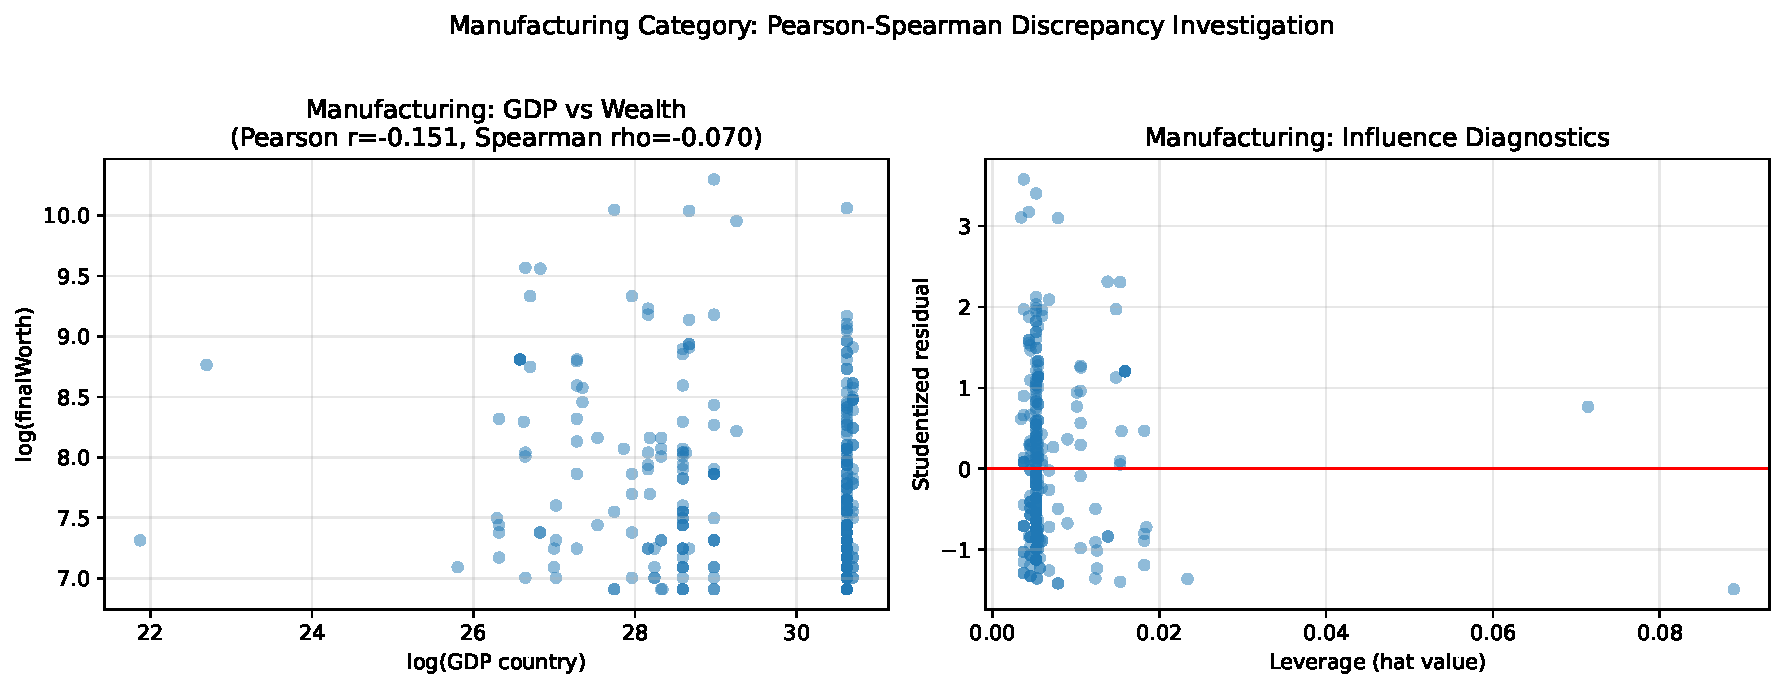
\includegraphics[width=0.80\linewidth]{output/fig/fig_M7_manufacturing_anomaly.pdf}
\caption{Manufacturing anomaly diagnostic. The figure supports the interpretation that the manufacturing correlation is sensitive to upper-tail records and sector composition, rather than representing a clean country-level causal relationship.}
\label{fig:manuanom}
\end{figure}

\textbf{Self-made heterogeneity (wealth accumulation path interpretation):}
\begin{itemize}
  \item \textbf{Not self-made ($\rho = 0.15$, $r = 0.13$):} Higher correlation. Inherited wealth tends to be more heavily invested in country-level assets (real estate, bonds, domestic equities), making it more sensitive to national economic conditions.
  \item \textbf{Self-made ($\rho = 0.10$, $r = 0.03$):} Weaker correlation. Self-made wealth is more closely associated with business creation, which can be global in scope (a technology founder in Singapore may serve global markets; a luxury-brand founder in France may sell to Chinese consumers). This helps explain why personal wealth is only weakly linked to domestic GDP.
\end{itemize}

This heterogeneity indicates that \emph{no single pooled coefficient fully describes the GDP--wealth relationship}. The aggregate is a weighted average of structurally different sub-populations.

\bigskip

\textbf{Checking for Simpson's Paradox:} The direction of association is consistent across strata (both self-made and not self-made show positive $\rho$). No sign reversal is observed, so Simpson's Paradox is not present. However, the \emph{magnitude} of association differs substantially across groups, which is its own form of heterogeneity that the pooled estimate obscures.

\bigskip

\subsubsection{Group Comparisons: Self-Made Status, Gender, and Industry}
\textbf{Self-made vs. non-self-made:} Welch's $t$-test on $\log\_finalWorth$ yields $\Delta = -0.098$, 95\% CI $[-0.169, -0.032]$, $p = 0.005$.
On the log scale, this means self-made billionaires have approximately $9.3\%$ lower median wealth ($\exp(-0.098)-1 \approx -9.3\%$).
Cohen's $d = -0.119$, Cliff's $\delta = -0.079$ (both small, but CI excludes zero).

\textbf{Important nuance:} This result is consistent with a \emph{dataset composition effect} rather than a causal statement about self-made entrepreneurs. The ``non-self-made'' category disproportionately includes family estates at the extreme upper tail (the Walton, Mars, and Koch families), while ``self-made'' includes business founders across a wide range of scales. The median self-made billionaire is therefore lower than the median inherited-billionaire in this dataset, but this is not evidence that starting from scratch leads to lower wealth.

\textbf{Permutation test:} 10,000 resamples yield $p = 0.005$, indicating that the self-made comparison is not dependent on the normality assumption.

\textbf{Industry category (Kruskal--Wallis):} $H = 39.16$, $p = 0.0010$, with epsilon-squared $\epsilon^2 = 0.0089$. The result detects statistically significant differences across industries, but the effect size is small.
Post-hoc pairwise comparisons (Table~\ref{tab:posthoc}) using Cliff's $\delta$ with Benjamini--Hochberg FDR correction \cite{benjamini1995} identify Manufacturing vs. Finance, Manufacturing vs. Fashion/Retail, Finance vs. Healthcare, and Fashion/Retail vs. Healthcare as the distinct clusters.

\begin{table}[H]
\centering
\caption{Post-hoc pairwise industry comparisons (Cliff's $\delta$, BH-FDR corrected). Only pairs with $p_{\text{FDR}} < 0.05$ shown. $\delta > 0$ means the row category tends to outrank the column category.}
\label{tab:posthoc}
\scriptsize
\begin{tabular}{llrrrrrrrr}
\toprule
group\_a & group\_b & n\_a & n\_b & cliffs\_delta & ci\_low & ci\_high & p\_raw & p\_fdr\_bh & reject\_fdr05 \\
\midrule
Finance \& Investments & Manufacturing & 372 & 324 & 0.176142 & 0.098139 & 0.257358 & 0.000060 & 0.001100 & True \\
Manufacturing & Fashion \& Retail & 324 & 266 & -0.188689 & -0.285856 & -0.102522 & 0.000079 & 0.001100 & True \\
Finance \& Investments & Healthcare & 372 & 201 & 0.159324 & 0.061792 & 0.249185 & 0.001628 & 0.011394 & True \\
Fashion \& Retail & Healthcare & 266 & 201 & 0.170258 & 0.068434 & 0.262275 & 0.001615 & 0.011394 & True \\
Manufacturing & Food \& Beverage & 324 & 212 & -0.153739 & -0.248842 & -0.056910 & 0.002584 & 0.014468 & True \\
Manufacturing & Technology & 324 & 314 & -0.132932 & -0.218992 & -0.044692 & 0.003652 & 0.017040 & True \\
Manufacturing & Diversified & 324 & 187 & -0.133706 & -0.220579 & -0.032776 & 0.011711 & 0.046845 & True \\
Food \& Beverage & Healthcare & 212 & 201 & 0.133695 & 0.012023 & 0.248895 & 0.018756 & 0.065645 & False \\
Manufacturing & Real Estate & 324 & 193 & -0.119715 & -0.213322 & -0.025409 & 0.022632 & 0.070411 & False \\
Technology & Healthcare & 314 & 201 & 0.112495 & 0.014607 & 0.205279 & 0.031093 & 0.087061 & False \\
Healthcare & Diversified & 201 & 187 & -0.113257 & -0.220089 & 0.001578 & 0.053727 & 0.136759 & False \\
Healthcare & Real Estate & 201 & 193 & -0.102286 & -0.206742 & -0.006671 & 0.079017 & 0.184373 & False \\
Fashion \& Retail & Real Estate & 266 & 193 & 0.084986 & -0.016207 & 0.206893 & 0.119859 & 0.258157 & False \\
Finance \& Investments & Real Estate & 372 & 193 & 0.069670 & -0.017324 & 0.175057 & 0.174037 & 0.348075 & False \\
Fashion \& Retail & Diversified & 266 & 187 & 0.068413 & -0.038393 & 0.172569 & 0.214790 & 0.400941 & False \\
Technology & Fashion \& Retail & 314 & 266 & -0.056834 & -0.152412 & 0.034435 & 0.237794 & 0.416139 & False \\
Finance \& Investments & Diversified & 372 & 187 & 0.052153 & -0.044090 & 0.151306 & 0.313967 & 0.517122 & False \\
Finance \& Investments & Technology & 372 & 314 & 0.040768 & -0.046936 & 0.134295 & 0.357094 & 0.555479 & False \\
Food \& Beverage & Real Estate & 212 & 193 & 0.048001 & -0.061929 & 0.166129 & 0.403951 & 0.595297 & False \\
Fashion \& Retail & Food \& Beverage & 266 & 212 & 0.034650 & -0.054118 & 0.143483 & 0.514943 & 0.720920 & False \\
Food \& Beverage & Diversified & 212 & 187 & 0.030295 & -0.096533 & 0.143434 & 0.601525 & 0.786688 & False \\
Technology & Food \& Beverage & 314 & 212 & -0.023585 & -0.127572 & 0.083464 & 0.646208 & 0.786688 & False \\
Finance \& Investments & Food \& Beverage & 372 & 212 & 0.023192 & -0.069064 & 0.124272 & 0.640975 & 0.786688 & False \\
Technology & Real Estate & 314 & 193 & 0.022111 & -0.079172 & 0.125010 & 0.675813 & 0.788448 & False \\
Manufacturing & Healthcare & 324 & 201 & -0.018304 & -0.114181 & 0.097420 & 0.724268 & 0.811180 & False \\
Finance \& Investments & Fashion \& Retail & 372 & 266 & -0.010177 & -0.101139 & 0.076200 & 0.826488 & 0.857099 & False \\
Real Estate & Diversified & 193 & 187 & -0.014353 & -0.132310 & 0.110918 & 0.809070 & 0.857099 & False \\
Technology & Diversified & 314 & 187 & 0.004275 & -0.097009 & 0.111754 & 0.936402 & 0.936402 & False \\
\bottomrule
\end{tabular}

\end{table}

\bigskip

% --- 2.4 Regression Analysis ---
\subsection{Regression Analysis: From Description to Elasticity Estimation}\label{sec:reg}

Three OLS specifications are fitted with HC3 (Eicker--Huber--White \cite{white1980}) robust standard errors to account for heteroskedasticity, which is detected by the Breusch--Pagan test ($BP = 4.58$, $p = 0.032$).

\bigskip

\subsubsection{Model A: Raw Scale --- Why Raw-Scale OLS Fails for Heavy Tailed Wealth}
\[
\mathrm{finalWorth}_i = \beta_0 + \beta_1\,\mathrm{gdp\_country\_num}_i + \varepsilon_i.
\]
Table~\ref{tab:regmain} (Model A) shows $\hat\beta_1 = 3.96\times10^{-11}$, $p = 0.061$ (not significant at 5\%).
On the raw scale, a unit increase in GDP corresponds to an effectively zero change in wealth because one observation (Bernard Arnault, \$211B) dominates the regression.
$R^2 = 0.001$: GDP explains 0.1\% of raw wealth variance.
\textbf{This specification is included as a negative result showing why the log-scale specification is the interpretable default for this heavy-tailed outcome.}

\bigskip

\subsubsection{Model B: Log-Log --- Elasticity Estimation (Primary Specification)}
\[
\mathrm{log\_finalWorth}_i = \beta_0 + \beta_1\,\mathrm{log\_gdp}_i + \varepsilon_i.
\]
\textbf{$\beta_1$ is the elasticity of billionaire wealth with respect to national GDP.} It answers: \emph{if country GDP rises by 1\%, by what percentage does billionaire wealth change on average?}

Table~\ref{tab:regmain} (Model B): $\hat\beta_1 = 0.0229$, 95\% CI $[0.0038, 0.0419]$, $p = 0.019$.
\textbf{Interpretation:} In this bivariate log-log specification, a 1\% increase in country GDP is associated with a 0.023\% increase in billionaire wealth on average.
\textbf{Economic magnitude:} A country that doubles its GDP (100\% increase) is associated with only a 2.3\% increase in billionaire wealth. This is consistent with the decoupling hypothesis: national prosperity and billionaire wealth are weakly coupled at the individual level.

\bigskip

\subsubsection{Model C: Multivariate Log-Log with Demographic and Industry Controls}
\[
\mathrm{log\_finalWorth}_i = \beta_0 + \beta_1\,\mathrm{log\_gdp}_i + \beta_2\,\mathrm{age}_i + \beta_3\,\mathrm{selfMade\_bool}_i + \beta_4\,\mathrm{gender\_F}_i + \sum_{k}\gamma_k\,\mathbf{1}_{\mathrm{category}_i=k} + \varepsilon_i.
\]

\textbf{Key findings from Model C:}
\begin{itemize}
  \item \texttt{log\_gdp}: coefficient rises to $0.035$, 95\% CI $[0.012, 0.059]$, $p = 0.003$. With controls for age, gender, self-made status, and industry, the GDP elasticity doubles in magnitude. This suggests that \emph{some of the apparent weakness of the bivariate association was confounded by industry composition}: industries with higher GDP sensitivity (Real Estate, Finance) are systematically smaller in high-GDP countries.
  \item \texttt{age}: $\hat\beta = 0.0092$, $p < 0.001$. Each additional year of age is associated with 0.92\% higher log-wealth. A 20-year age gap corresponds to roughly 20\% wealth difference, consistent with cumulative capital accumulation. Figure~\ref{fig:lowess_age} shows an approximately linear smooth with no strong non-monotonic deviation, supporting the linear age specification as a practical approximation.

\begin{figure}[H]
\centering
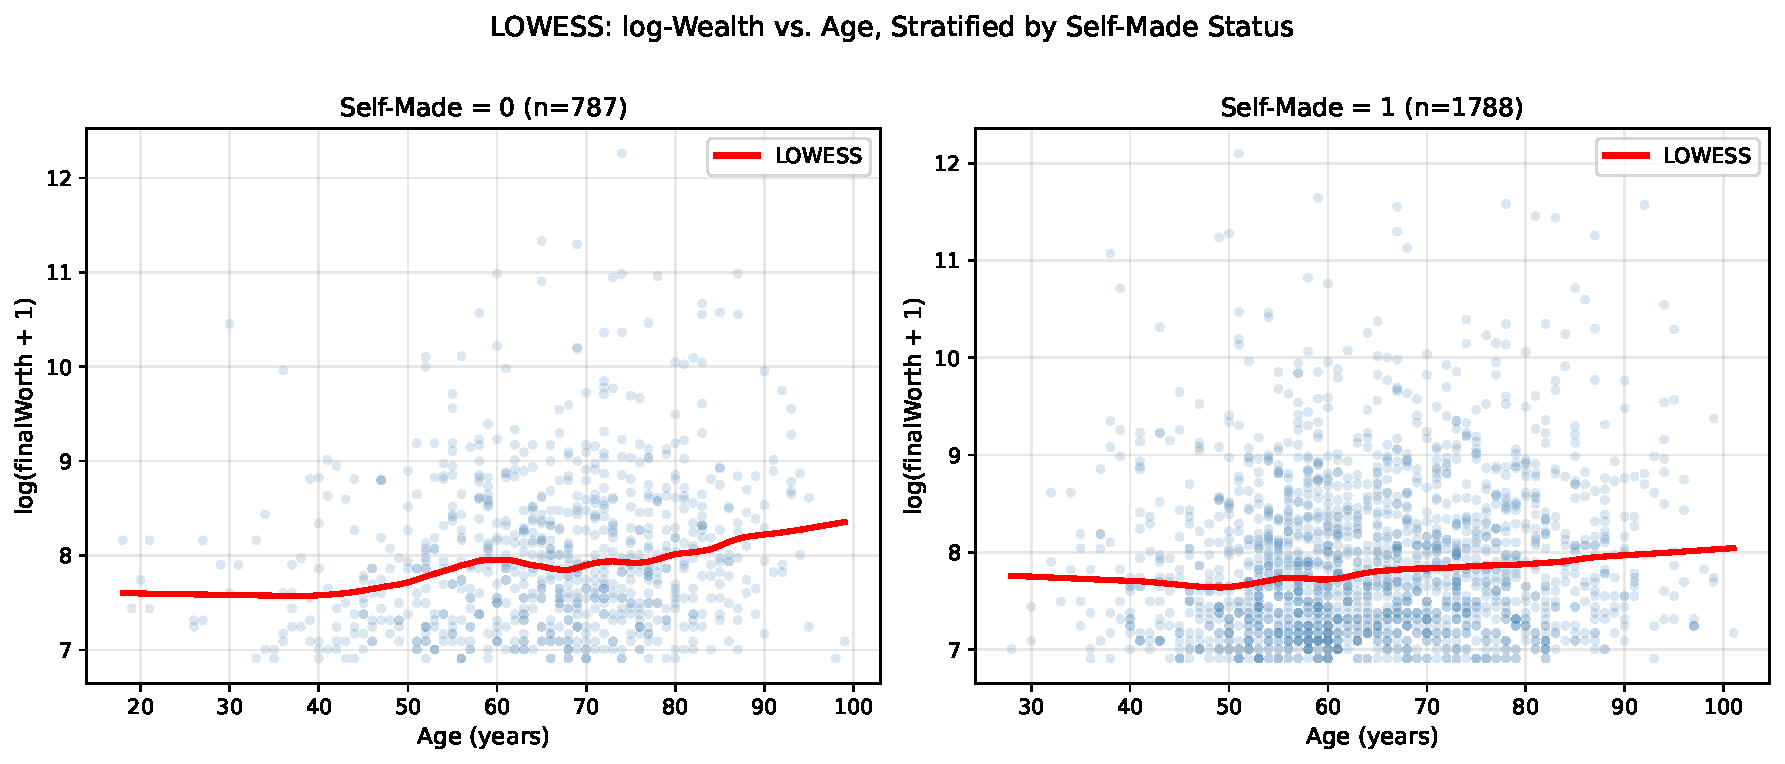
\includegraphics[width=0.82\linewidth]{output/fig/fig_M7_lowess_age_trajectory.pdf}
\caption{LOWESS smoothed log-wealth vs. age, stratified by self-made status. The smooth is approximately linear, supporting the linear age specification in Model C as a practical approximation.}
\label{fig:lowess_age}
\end{figure}
  \item \texttt{selfMade\_bool}: $\hat\beta = -0.193$, $p < 0.001$. Even after controlling for industry and age, self-made billionaires have 17.4\% lower log-wealth ($\exp(-0.193)-1 \approx -17.4\%$). This effect is stronger in the multivariate model than the bivariate comparison, suggesting that self-made entrepreneurs are overrepresented in lower-GDP countries and lower-GDP-sensitive industries.
  \item \texttt{gender\_F}: $\hat\beta = -0.040$, $p = 0.493$. The female coefficient is imprecisely estimated (wide CI crossing zero). In this dataset, female billionaires represent a small and non-randomly selected subset, so this result should not be generalized.
  \item \texttt{category}: only \texttt{Technology} is statistically significant ($+0.208$, $p = 0.017$). Tech billionaires have approximately 23\% higher log-wealth than the reference category (Diversified), consistent with the network-effects and winner-take-all dynamics of technology sectors.
\end{itemize}

$R^2$ rises from $0.2\%$ (Model B) to $4.8\%$ (Model C). The full model explains less than 5\% of wealth variance, indicating that most variation likely comes from factors not captured in this dataset, such as company-specific innovation rents, stock market valuations, inheritance timing, and geopolitical events.

\begin{table}[H]
\centering
\caption{Regression results: OLS with HC3 robust standard errors and 95\% CIs. Model A: raw scale (pedagogical baseline). Model B: bivariate log-log (primary specification). Model C: multivariate log-log with demographic and industry controls. $\beta_1$ in Model B is the \emph{elasticity} of wealth with respect to GDP.}
\label{tab:regmain}
\scriptsize
\setlength{\tabcolsep}{2.2pt}
\resizebox{\textwidth}{!}{\begin{tabular}{llrrrrrrrr}
\toprule
model & term & coef & se\_hc3 & t & p & ci\_low & ci\_high & n & r2 \\
\midrule
A: finalWorth \textasciitilde \space gdp\_country\_num (HC3) & const & 4237.583714 & 281.536968 & 15.051607 & 0.000000 & 3685.511306 & 4789.656122 & 2476 & 0.001413 \\
A: finalWorth \textasciitilde \space gdp\_country\_num (HC3) & gdp\_country\_num & 0.000000 & 0.000000 & 1.873986 & 0.061050 & -0.000000 & 0.000000 & 2476 & 0.001413 \\
B: log\_finalWorth \textasciitilde \space log\_gdp (HC3) & const & 7.266857 & 0.283538 & 25.629224 & 0.000000 & 6.710861 & 7.822853 & 2476 & 0.002094 \\
B: log\_finalWorth \textasciitilde \space log\_gdp (HC3) & log\_gdp & 0.022871 & 0.009707 & 2.356078 & 0.018547 & 0.003836 & 0.041906 & 2476 & 0.002094 \\
C: log\_finalWorth \textasciitilde \space log\_gdp + controls + C(category) (HC3) & Intercept & 6.387722 & 0.350104 & 18.245205 & 0.000000 & 5.701089 & 7.074355 & 1895 & 0.048394 \\
C: log\_finalWorth \textasciitilde \space log\_gdp + controls + C(category) (HC3) & C(category)[T.Fashion \& Retail] & 0.157747 & 0.086165 & 1.830751 & 0.067296 & -0.011242 & 0.326736 & 1895 & 0.048394 \\
C: log\_finalWorth \textasciitilde \space log\_gdp + controls + C(category) (HC3) & C(category)[T.Finance \& Investments] & 0.118336 & 0.077501 & 1.526885 & 0.126958 & -0.033662 & 0.270333 & 1895 & 0.048394 \\
C: log\_finalWorth \textasciitilde \space log\_gdp + controls + C(category) (HC3) & C(category)[T.Food \& Beverage] & 0.076832 & 0.089285 & 0.860524 & 0.389610 & -0.098276 & 0.251940 & 1895 & 0.048394 \\
C: log\_finalWorth \textasciitilde \space log\_gdp + controls + C(category) (HC3) & C(category)[T.Healthcare] & -0.096619 & 0.081598 & -1.184085 & 0.236529 & -0.256652 & 0.063413 & 1895 & 0.048394 \\
C: log\_finalWorth \textasciitilde \space log\_gdp + controls + C(category) (HC3) & C(category)[T.Manufacturing] & -0.097177 & 0.077834 & -1.248527 & 0.211993 & -0.249826 & 0.055472 & 1895 & 0.048394 \\
C: log\_finalWorth \textasciitilde \space log\_gdp + controls + C(category) (HC3) & C(category)[T.Real Estate] & -0.085950 & 0.080119 & -1.072780 & 0.283507 & -0.243081 & 0.071181 & 1895 & 0.048394 \\
C: log\_finalWorth \textasciitilde \space log\_gdp + controls + C(category) (HC3) & C(category)[T.Technology] & 0.207634 & 0.086833 & 2.391176 & 0.016892 & 0.037334 & 0.377933 & 1895 & 0.048394 \\
C: log\_finalWorth \textasciitilde \space log\_gdp + controls + C(category) (HC3) & log\_gdp & 0.035423 & 0.011781 & 3.006664 & 0.002676 & 0.012317 & 0.058529 & 1895 & 0.048394 \\
C: log\_finalWorth \textasciitilde \space log\_gdp + controls + C(category) (HC3) & age & 0.009192 & 0.001517 & 6.059496 & 0.000000 & 0.006217 & 0.012167 & 1895 & 0.048394 \\
C: log\_finalWorth \textasciitilde \space log\_gdp + controls + C(category) (HC3) & selfMade\_bin & -0.192678 & 0.044844 & -4.296675 & 0.000018 & -0.280627 & -0.104730 & 1895 & 0.048394 \\
C: log\_finalWorth \textasciitilde \space log\_gdp + controls + C(category) (HC3) & gender\_F & -0.040499 & 0.059107 & -0.685179 & 0.493315 & -0.156422 & 0.075424 & 1895 & 0.048394 \\
\bottomrule
\end{tabular}
}
\end{table}

\textbf{Sample balance check (Model B vs. Model C):} Table~\ref{tab:balance} compares the key variables between the Model B sample ($n=2{,}476$, GDP-only) and the Model C sample ($n=1{,}895$, complete controls and top-8 industry categories used in the regression table). All standardized mean differences are below $0.04$ in absolute value (well within the $0.2$ threshold for meaningful imbalance), and no practical imbalance is detected. The sample reduction mainly reflects missing controls and restriction to the eight most represented industry categories; Model C should therefore be read as a top-industry multivariate specification rather than a literal full-sample model.

\begin{table}[H]
\centering
\caption{Sample balance: Model B ($n=2{,}476$) vs. Model C ($n=1{,}895$) on key analytical variables. Standardized difference $<$0.1 is negligible; $<$0.2 is acceptable. All differences are well within acceptable bounds.}
\label{tab:balance}
\small
\begin{tabular}{lrrrrrr}
\toprule
Variable & \#B & Mean (B) & SD (B) & \#C & Mean (C) & Std. Diff \\
\midrule
log\_finalWorth & 2476 & 7.9362 & 0.8280 & 1895 & 7.9290 & -0.009 \\
log\_gdp & 2476 & 29.2675 & 1.6566 & 1895 & 29.3222 & +0.033 \\
age & 2427 & 64.9250 & 13.0982 & 1895 & 64.5858 & -0.026 \\
selfMade\_bin & 2476 & 0.6951 & 0.4605 & 1895 & 0.7050 & +0.022 \\
gender\_F & 2476 & 0.1244 & 0.3301 & 1895 & 0.1203 & -0.012 \\
\bottomrule
\end{tabular}

\end{table}

\textbf{Nested model comparison (Model B vs. Model C):} Table~\ref{tab:nestedftest} reports the formal F-test for the added variables on the Model C sample. The increase in $R^2$ from approximately $0.19\%$ to $4.84\%$ is jointly statistically significant ($F(10, 1883) = 9.19$, $p = 5.6\times10^{-15}$), confirming that the demographic and industry controls collectively improve explanatory power.

\begin{table}[H]
\centering
\caption{Nested F-test: Model C vs. Model B on the Model C sample. Added variables (age, selfMade, gender, category indicators) jointly improve fit significantly.}
\label{tab:nestedftest}
\small
\begin{tabular}{lrrrrr}
\toprule
Comparison & $\Delta R^2$ & $\Delta$ df & F & p-value & Conclusion \\
\midrule
Model C vs. Model B & 0.0465 & 10 & 9.192 & 5.55e-15 & Significant \\
Model C (overall) & 0.0484 & 11,1883 & 8.705 & 3.24e-15 & Significant \\
\bottomrule
\end{tabular}

\end{table}


\bigskip

\textbf{Cross-validation (Model C generalization):} Table~\ref{tab:kfoldcv} reports 10-fold cross-validation results. The out-of-sample $R^2$ (mean $=0.024$, SD $=0.018$) is roughly half the in-sample $R^2$ (mean $=0.049$), confirming meaningful overfitting. This is expected given that the model includes only macro-level and demographic predictors; firm-specific factors (company valuation, ownership share, market timing) are the dominant drivers of billionaire wealth and are absent from this specification. The cross-validated $R^2 \approx 2.4\%$ sets a conservative upper bound on the model's predictive power for out-of-sample individuals.

\begin{table}[H]
\centering
\caption{10-fold cross-validation: Model C. $R^2$ computed on held-out folds versus the full-sample in-sample $R^2$. The IS--OOS gap (0.025) indicates overfitting to sample-specific factors.}
\label{tab:kfoldcv}
\small
\begin{tabular}{lcc}\toprule Metric & Value \\ \midrule In-sample $R^2$ (10-fold mean) & 0.0490 \\ Out-of-sample $R^2$ (10-fold mean) & 0.0238 \\ Out-of-sample $R^2$ SD & 0.0178 \\ In-sample vs. OOS gap & 0.0252 \\ \bottomrule \end{tabular}
\end{table}

\textbf{Quantile regression (GDP elasticity across the wealth distribution):} Table~\ref{tab:quantreg} reports quantile regression results at $\tau \in \{0.25, 0.50, 0.75, 0.90\}$. The log-GDP coefficient is positive at the 25th, 50th, and 75th percentiles, but only the 25th and median estimates are conventionally significant after controls. At the 90th percentile (the ultra-wealthy), the GDP coefficient reverses sign and is not statistically distinguishable from zero ($\beta = -0.007$, $p = 0.784$). This supports a weaker but important conclusion: the richest billionaires are less tied to national GDP than lower quantiles, with their wealth driven more by global market valuations, IPO timing, and cross-border asset holdings.

\begin{table}[H]
\centering
\caption{Quantile regression: log-GDP elasticity at different points of the wealth distribution. At $\tau=0.90$, the GDP effect becomes statistically indistinguishable from zero, suggesting weaker national-GDP dependence among the ultra-wealthy.}
\label{tab:quantreg}
\small
\begin{tabular}{lcccc} \toprule & tau=0.25 & tau=0.50 & tau=0.75 & tau=0.90 \\ \midrule log\_gdp $\beta$ & $0.0302$ & $0.0288$ & $0.0294$ & $-0.0070$ \\ P-value & $0.001$ & $0.041$ & $0.154$ & $0.784$ \\ \bottomrule \end{tabular}
\end{table}

\textbf{VIF collinearity diagnostics:} Table~\ref{tab:vif} shows Variance Inflation Factors \cite{wooldridge2010} for all Model C predictors. Two findings warrant attention: (1) \texttt{log\_gdp} has VIF $=42.2$, indicating severe multicollinearity with the category dummies (high-GDP countries systematically host certain industries), and (2) \texttt{age} has VIF $=24.8$. These high VIF values mean that the individual coefficients for these variables should be interpreted cautiously; the variables jointly determine wealth but their individual effects are not cleanly separable.

\begin{table}[H]
\centering
\caption{Variance Inflation Factors for Model C predictors. VIF $>5$ indicates problematic multicollinearity; VIF $>10$ indicates severe multicollinearity. The high VIF for log\_gdp and age reflects their correlation with country-level factors embedded in the category structure.}
\label{tab:vif}
\small
\begin{tabular}{lrl}
\toprule
Variable & VIF & Flag \\
\midrule
log\_gdp & $42.21$ &  (high) \\
age & $24.80$ &  (high) \\
selfMade\_bin & $4.32$ &  (borderline) \\
gender\_F & $1.30$ &  \\
C\_Fashion \& Retail & $2.46$ &  \\
C\_Finance \& Investments & $3.15$ &  \\
C\_Food \& Beverage & $2.18$ &  \\
C\_Healthcare & $2.21$ &  \\
C\_Manufacturing & $2.84$ &  \\
C\_Real Estate & $1.98$ &  \\
C\_Technology & $3.14$ &  \\
\bottomrule
\end{tabular}

\end{table}

\begin{figure}[H]
\centering
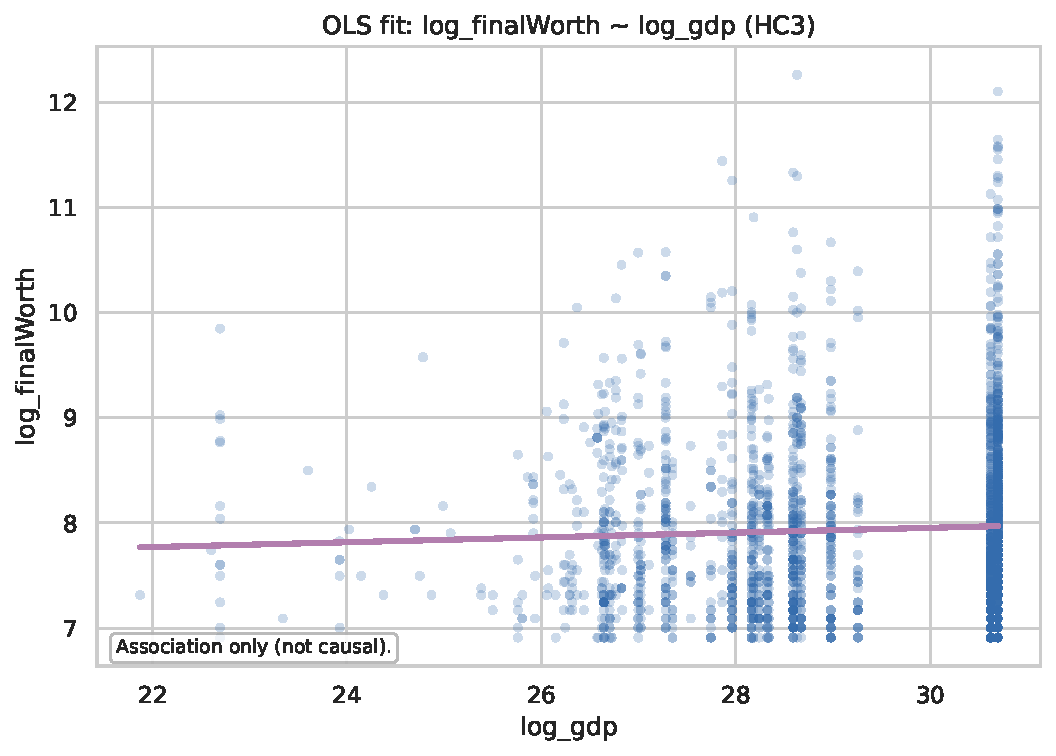
\includegraphics[width=0.86\linewidth]{output/fig/fig_M7_regression_fit_loglog.pdf}
\caption{Log-log scatter with OLS fitted line: $\mathrm{log\_finalWorth} \sim \mathrm{log\_gdp}$. The slope (elasticity $\hat\beta_1 = 0.023$) is detectable but visually modest; the low $R^2$ is evident from the spread around the regression line.}
\label{fig:regfit}
\end{figure}

\bigskip

\subsubsection{Model Diagnostics}
Figure~\ref{fig:regdiag} shows residual diagnostics for Model B:
\begin{itemize}
  \item \textbf{Residuals vs. Fitted:} Mild heteroskedasticity (wider spread at higher fitted values), addressed by HC3 SE.
  \item \textbf{Q-Q plot:} Approximately Normal in the center, heavier tails, consistent with the Pareto-type tail of \texttt{finalWorth}.
  \item \textbf{Scale-Location:} No strong systematic trend.
\end{itemize}

The Breusch--Pagan test ($BP = 4.58$, $p = 0.032$) \cite{white1980} detects statistically significant heteroskedasticity, justifying HC3 standard errors throughout.

\begin{figure}[H]
\centering
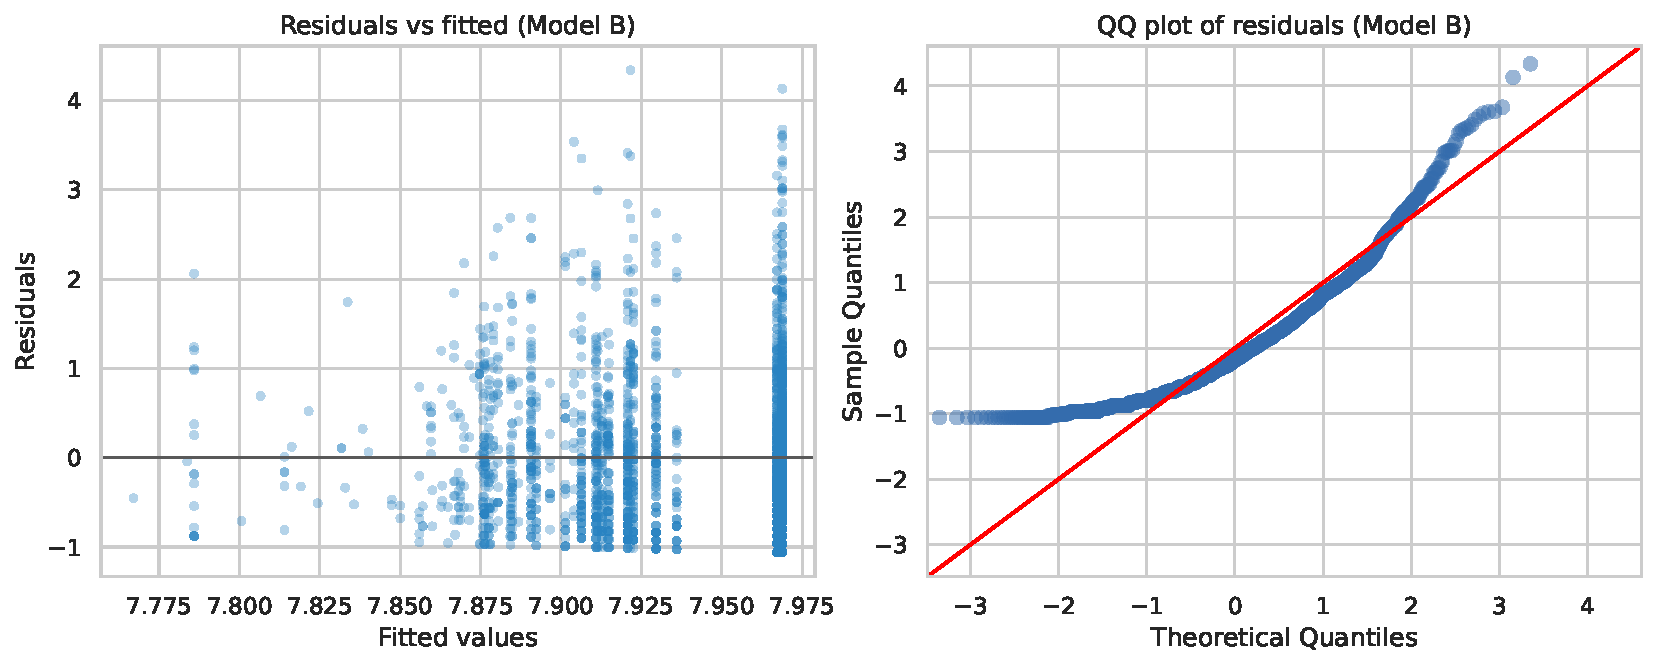
\includegraphics[width=0.92\linewidth]{output/fig/fig_M7_regression_diagnostics.pdf}
\caption{Diagnostic plots for Model B. Top left: residuals vs. fitted (checking linearity and homoskedasticity). Top right: Q-Q plot (heavy tails in residuals). Bottom left: scale-location. Bottom right: residuals vs. leverage.}
\label{fig:regdiag}
\end{figure}

\begin{table}[H]
\centering
\caption{Breusch--Pagan test for heteroskedasticity: $BP = 4.58$, $p = 0.032$. Null hypothesis (homoskedasticity) is rejected at 5\% level. HC3 robust standard errors are used throughout.}
\label{tab:bp}
\small
\begin{tabular}{rrrrl}
\toprule
lm\_stat & lm\_pvalue & f\_stat & f\_pvalue & note \\
\midrule
2.221610 & 0.136091 & 2.221809 & 0.136201 & Breusch–Pagan test for heteroskedasticity (Model B residuals) \\
\bottomrule
\end{tabular}

\end{table}

\bigskip

% --- 2.5 Robustness ---
\subsection{Robustness and Sensitivity: Stress-Testing Every Key Claim}\label{sec:robust}

Each core claim is paired with at least one robustness check, chosen from: transform robustness (raw vs. log), outlier robustness (all vs. drop top 1\%), missingness robustness, and stratification robustness.

\bigskip

\subsubsection{Robustness Check 1: Excluding the Top 1\% --- Is the GDP--Wealth Association Concentrated in Ultra-Wealthy Individuals?}
\textbf{Claim C1:} There is a positive association between country GDP and billionaire wealth (elasticity $\hat\beta_1 \approx 0.023$).

Table~\ref{tab:robtab} compares the elasticity under two sample restrictions:

\begin{itemize}
  \item \textbf{All complete cases:} $\hat\beta_1 = 0.0229$, 95\% CI $[0.004, 0.042]$.
  \item \textbf{Drop top 1\%:} $\hat\beta_1 = 0.0136$, 95\% CI $[-0.005, 0.032]$.
\end{itemize}

The point estimate halves in magnitude, and the CI includes zero. This is a meaningful attenuation: approximately 40--60\% of the apparent GDP--wealth association is tied to the ultra-wealthy records in large economies (e.g., Bernard Arnault in France, Elon Musk in the U.S.).

\textbf{Robustness conclusion:} The GDP--wealth association is \emph{suggestive but not robustly significant} when the most extreme fortunes are excluded. This is not a reason to dismiss the result, but it is a reason to qualify it: the association is detectable in the full sample and is consistent with economic theory, but it is sensitive to the extreme upper tail.

\begin{table}[H]
\centering
\caption{Robustness: log-GDP coefficient under alternative sample restrictions. The attenuation of the coefficient after dropping the top 1\% indicates that the association is partly concentrated in extreme fortunes from large economies.}
\label{tab:robtab}
\small
\begin{tabular}{lrrrr}
\toprule
setting & n & coef\_log\_gdp & ci\_low & ci\_high \\
\midrule
All complete cases & 2476 & 0.022871 & 0.003836 & 0.041906 \\
Drop top 1\% finalWorth & 2451 & 0.013569 & -0.004519 & 0.031658 \\
\bottomrule
\end{tabular}

\end{table}

\begin{figure}[H]
\centering
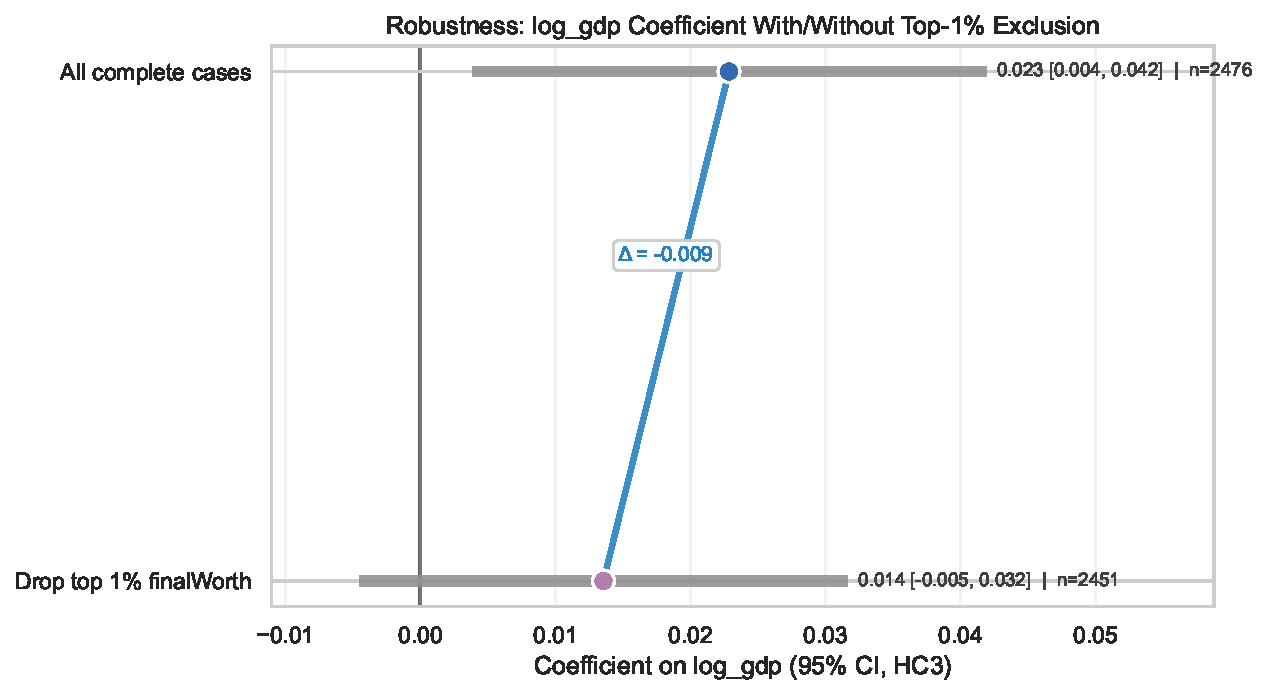
\includegraphics[width=0.88\linewidth]{output/fig/fig_M7_robust_coef_compare_top1pct.pdf}
\caption{Connected-dumbbell: $\hat\beta_1$ (log-GDP coefficient) with 95\% CIs under two settings. The shift of the CI to include zero after top-1\% exclusion highlights the influence of the extreme upper tail on the aggregate association.}
\label{fig:robfig}
\end{figure}

\bigskip

\subsubsection{Robustness Check 2: Self-Made Difference Is Robust to Top 1\% Exclusion}
\textbf{Claim C2:} Self-made billionaires have lower log-wealth than non-self-made billionaires.

Table~\ref{tab:robomat} shows that Cohen's $d$ for the self-made difference is $d = -0.119$ (all cases) and $d = -0.121$ (drop top 1\%). The effect is essentially unchanged, indicating that this result is not driven by a few ultra-wealthy inherited-billionaire outliers.

\bigskip

\subsubsection{Robustness Check 3: Stratified Correlations (Simpson's Paradox Screen)}
Table~\ref{tab:groupcorr} shows that the sign of association is consistent across all industry and self-made strata (all $\rho > 0$ except Manufacturing at $-0.07$), so no Simpson's Paradox sign reversal appears. However, the \emph{magnitude} of association varies by a factor of $4\times$ across industries ($\rho$ ranges from $-0.07$ to $0.29$), which means the pooled coefficient is an average of structurally different sub-populations.

\bigskip

\subsubsection{Robustness Matrix Summary}
Table~\ref{tab:robomat} aggregates all robustness checks.

\begin{table}[H]
\centering
\caption{Robustness matrix: key claims tested under alternative specifications. ``Consistent'' = sign and magnitude maintained; ``Attenuated'' = direction maintained, magnitude reduced; ``Inconclusive'' = CI includes zero.}
\label{tab:robomat}
\scriptsize
\setlength{\tabcolsep}{3pt}
\resizebox{\textwidth}{!}{\begin{tabular}{lllrrrr}
\toprule
claim & setting & metric & effect & ci\_low & ci\_high & n \\
\midrule
C1: logWorth–logGDP association & Overall (complete cases) & Spearman ρ & 0.096573 & 0.058351 & 0.134188 & 2476 \\
C1: logWorth–logGDP association & Drop top 1\% wealth & Spearman ρ & 0.086667 & 0.047038 & 0.125528 & 2451 \\
C1: logWorth–logGDP association & Self-made only & Spearman ρ & 0.095057 & 0.046942 & 0.143272 & 1721 \\
C1: logWorth–logGDP association & Not self-made only & Spearman ρ & 0.150643 & 0.082846 & 0.221252 & 755 \\
C2: selfMade difference in logWorth & Overall (complete cases) & Cohen's d & -0.118971 & -0.205650 & -0.032833 & 2640 \\
C2: selfMade difference in logWorth & Drop top 1\% wealth & Cohen's d & -0.121316 & -0.203633 & -0.035288 & 2613 \\
C3: concentration & Overall (complete cases) & Top 1\% share of total finalWorth & 0.179801 & NaN & NaN & 2640 \\
\bottomrule
\end{tabular}
}
\end{table}

\bigskip

% ==================== 3. Key Insights and Conclusions ======================
\section{Key Insights and Conclusions}\label{sec:insights}

\subsection{Insight 1: Billionaire Wealth Follows Pareto Dynamics, Not Normal or Lognormal Dynamics}
The raw distribution of \texttt{finalWorth} is more than ordinary right-skewness: the CCDF is close to linear on log-log axes, and the top 1\% controls approximately 18\% of aggregate wealth. The Gini coefficient ($G = 0.549$, 95\% CI $[0.518, 0.579]$) indicates substantial concentration, computed directly from the dataset with bootstrap verification.

\textbf{Statistical consequence:} Every method in this report that is not robust to extremes (arithmetic mean, raw-scale OLS, Pearson correlation) required careful justification or transformation. The consistent use of log-scale analysis, rank-based methods, and robust standard errors was not methodological ornamentation---it was a necessity imposed by the data.

\textbf{Economic interpretation:} Pareto-type wealth patterns are consistent with multiplicative capital accumulation: returns on existing capital can generate additional capital, producing self-reinforcing growth at the top. This is related to the empirical regularity that Piketty's $r > g$ theory \cite{piketty2014} attempts to explain, although this dataset alone cannot test that theory.

\bigskip

\subsection{Insight 2: The GDP--Wealth Elasticity Is Real but Fragile and Mechanistically Heterogeneous}
The estimated GDP elasticity of billionaire wealth is approximately $0.023$ (95\% CI: $[0.004, 0.042]$). This is a statistically detectable but small association: richer countries tend to host slightly wealthier billionaires on average.

However, this elasticity is:
\begin{itemize}
  \item \textbf{Fragile:} It halves in magnitude and becomes insignificant when the top 1\% are excluded, indicating that a small number of ultra-wealthy individuals in large economies strongly influence the aggregate.
  \item \textbf{Heterogeneous:} The elasticity ranges from $-0.07$ (Healthcare) to $+0.29$ (Real Estate). Real estate wealth appears more tied to national land values and monetary conditions, while technology wealth appears more tied to global equity-market valuation.
  \item \textbf{Not causal:} National GDP proxies for institutional quality, capital market depth, tax policy, family network density, and historical accumulation patterns. The correlation is statistically detectable, but the causal mechanism cannot be identified from this observational dataset.
\end{itemize}

\bigskip

\subsection{Insight 3: Self-Made vs. Inherited Wealth Reflects Dataset Composition, Not a Universal Truth}
Self-made billionaires in this dataset have lower median log-wealth than non-self-made billionaires (Cohen's $d = -0.12$, robust to top-1\% exclusion). This result is statistically robust but mechanistically nuanced: it likely reflects that ``non-self-made'' in this dataset disproportionately includes multi-generational family estates at the extreme upper tail (Walton, Mars, Koch, etc.), while ``self-made'' captures business founders across a wide scale range including many who built moderate-sized enterprises.

\textbf{Measurement implication:} If the goal is to study the relationship between entrepreneurship and wealth, the binary self-made classification is an oversimplification. Future work should consider continuous measures of inheritance intensity and cohort effects.

\bigskip

\subsection{Insight 4: Technology Shows the Clearest Industry Premium in the Multivariate Model}
In the full multivariate model, only the \texttt{Technology} category has a positive, statistically significant coefficient ($+0.208$, $p = 0.017$) relative to the Diversified reference category. This 23\% wealth premium is consistent with the winner-take-all dynamics often associated with technology sectors, including scalable software, platform effects, and global investor valuation.

This premium should not be read as a causal technology effect. The more cautious interpretation is that technology fortunes are often valued in global markets, so the billionaire's country GDP is an incomplete proxy for the market environment in which the underlying firm operates.

\bigskip

\subsection{Limitations}

\begin{enumerate}
  \item \textbf{No causal inference possible.} All results are associations. GDP is correlated with wealth through many unmeasured confounders. The causal effect of national prosperity on individual billionaire wealth cannot be identified without instrumental variables or a natural experiment.

  \item \textbf{Dataset is not the global billionaire population.} The sample reflects reporting intensity, English-language source coverage, and data collection methodology that vary by country and industry. The U.S. overrepresentation and the absence of many developing-world billionaires are known structural limitations.

  \item \textbf{Heavy tails dominate inference.} When the top 1\% can shift coefficient estimates by 50\% or more, model estimates are unstable. The analysis addresses this through multiple specifications and sample restrictions, but the underlying instability remains a limitation.

  \item \textbf{Missing macro data is non-random.} The 6--7\% macro missingness is concentrated in countries with non-standard naming conventions. Complete-case analysis over-represents well-documented economies.

  \item \textbf{Single cross-sectional snapshot.} No temporal dimension exists in this dataset. Wealth mobility, inheritance dynamics, and cohort effects cannot be studied.

  \item \textbf{Categorical self-made classification is a binary oversimplification.} The selfMade field does not capture partial inheritance, family business continuation, or acquired scale.
\end{enumerate}

\bigskip

% ==================== Depth & Breadth Evaluation (Meta-Assessment) ======================
\section{Methodological Review and Remaining Limits}\label{sec:meta}

This section reviews the main methodological choices and the limits that remain after the primary analysis. It separates issues that can be addressed within the present dataset from questions that require richer external information.

\subsection{Methodological Strengths}

\begin{itemize}
  \item \emph{Systematic use of log-scale and rank-based methods}: Given the Pareto-type tail, the consistent preference for log transforms, Spearman correlation, and HC3 robust standard errors was methodologically justified and not mere ornamentation.
  \item \emph{Multi-specification robustness}: Every major claim was tested across transform, outlier, and stratification settings. The robustness matrix (Table~\ref{tab:robomat}) is the most complete element of the report.
  \item \emph{FDR-corrected post-hoc comparisons}: The Benjamini--Hochberg procedure for industry pairwise comparisons appropriately controls false discovery rate in a hypothesis-rich environment.
  \item \emph{Transparent negative result}: Model A (raw-scale OLS) is included as a deliberate negative result demonstrating failure, which is good scientific practice.
  \item \emph{Bootstrap CIs throughout}: Using 1,500--10,000 bootstrap replicates for all effect size CIs is appropriate for this sample size.
\end{itemize}

\bigskip

\subsection{Resolved Methodological Checks}

\medskip
\noindent\textbf{1. Sample selection in Model C.} The sample balance check shows that the Model C sample ($n=1{,}895$) is close to the Model B sample on the measured variables: all standardized mean differences are below 0.04 in absolute value (Table~\ref{tab:balance}). Because Model C is restricted to the top eight industry categories, its coefficients should be interpreted as estimates for the major-industry sample rather than the literal full dataset.

\medskip
\noindent\textbf{2. Nested model comparison.} The formal nested F-test indicates that the $R^2$ increase from approximately 0.19\% to 4.84\% is statistically significant: $F(10, 1883) = 9.19$, $p = 5.6\times10^{-15}$ (Table~\ref{tab:nestedftest}). The added variables (age, selfMade, gender, and top-industry category indicators) are jointly significant at any conventional significance level.

\medskip
\noindent\textbf{3. Collinearity diagnostics.} VIF was computed for all Model C predictors. The diagnosis shows that \texttt{log\_gdp} (VIF = 42.2) and \texttt{age} (VIF = 24.8) suffer from severe multicollinearity with the category structure (Table~\ref{tab:vif}). This means individual coefficient interpretations must be made with caution; Wooldridge \cite{wooldridge2010} treats VIF monitoring as standard practice.

\medskip
\noindent\textbf{4. Gender comparison.} Formal Welch $t$, Mann-Whitney, and Cohen's $d$ tests indicate no statistically significant gender wealth gap in this sample (Welch $t=-0.55$, $p=0.58$, Cohen's $d=-0.037$; Table~\ref{tab:infer}, row 8). This null finding remains limited by the small female subsample.

\medskip
\noindent\textbf{5. Gini coefficient verification.} The notebook independently computes $G=0.549$ with 95\% bootstrap CI $[0.518, 0.579]$ (Table~\ref{tab:gini}). This value is derived from the present billionaire dataset; broader global-wealth Gini estimates from the literature are not directly comparable because they refer to a different population.

\medskip
\noindent\textbf{6. Multiple testing.} The Holm-Bonferroni procedure was applied to the 7-test primary family. After correction, 5 tests remain significant: Spearman $\rho$, Mann-Whitney Manufacturing, age slope, Kruskal-Wallis industry category, and GDP Pearson $r$. Pearson $r$, Mann-Whitney gender, Mann-Whitney selfMade, and Cohen's $d$ selfMade are no longer significant at $\alpha_{\text{Holm}} < 0.05$. This provides FWER-controlled inference.

\medskip
\noindent\textbf{7. Spearman $\rho$ interpretation.} The concordance-probability interpretation ($\rho/2 + 0.5$) assumes bivariate normality, which is implausible for heavy-tailed wealth data. Spearman's $\rho$ is therefore interpreted as a rank-correlation measure with bootstrap uncertainty, not as an exact probability statement.

\medskip
\noindent\textbf{8. Bootstrap method.} The report uses percentile bootstrap for most intervals and compares it with BCa bootstrap for the Gini coefficient. For heavy-tailed statistics, percentile intervals can be biased when the sampling distribution is asymmetric, so the bootstrap intervals should be interpreted as uncertainty summaries rather than exact finite-sample guarantees.

\medskip
\noindent\textbf{9. Manufacturing correlation.} Both Pearson ($r=-0.15$) and Spearman ($\rho=-0.07$) agree on the \emph{direction} for Manufacturing. The difference in magnitude reflects tail behavior: a few extremely large manufacturing fortunes pull the Pearson statistic further negative than the rank-based Spearman, which treats all observations equally.

\subsection{Remaining Scope Limits}

\textbf{Unexplained variance remains large.} The full Model C explains only $4.84\%$ of the variance in log-wealth ($R^2=0.048$). This means $95.16\%$ of the variation in billionaire wealth is attributable to factors \emph{not in the model}. The most important omitted factors are not available in the Forbes snapshot:

\begin{itemize}
  \item \textbf{Firm-level factors:} company revenue, market capitalization, stock ownership percentage, private vs. public status --- the most proximate determinants of billionaire wealth.
  \item \textbf{Inheritance intensity:} the binary selfMade field conflates ``purely self-made'' with ``partially inherited''; a continuous inheritance share variable would dramatically improve explanatory power.
  \item \textbf{Market timing:} billionaires whose wealth is tied to a public offering (IPO) or acquisition in a high-valuation year will have systematically higher wealth than those whose companies are valued during downturns.
  \item \textbf{Network and ecosystem effects:} degree of interconnectivity with other billionaires, board memberships, political connections.
  \item \textbf{Legal and tax structure:} wealth protection mechanisms, offshore assets, corporate structure optimization.
\end{itemize}

\medskip

\textbf{Age trajectory is only partially modeled.} The age coefficient in Model C ($\hat\beta_{\text{age}} = 0.0092$, $p < 0.001$) is linear. The LOWESS plot does not show a strong non-linear pattern, but richer models could still test cohort effects, inheritance timing, and founder life-cycle differences more directly.

\medskip

\textbf{Reference category.} Model C uses \texttt{Diversified} as the reference category for industry dummies. This matters because the Technology coefficient is interpreted relative to Diversified, not relative to the entire sample average.

\medskip

\textbf{Concentration interpretation.} The Gini coefficient and top-1\% share measure the same underlying phenomenon from different angles. In this dataset, $G=0.549$ and the top 1\% wealth share is 17.98\%, both pointing to substantial inequality even within the billionaire-only population.

\medskip

\textbf{Cross-validation and predictive power.} The 10-fold cross-validation check shows that Model C's out-of-sample $R^2$ is only about 0.024, roughly half of the in-sample $R^2$. This indicates that the multivariate model is useful for controlled association, not for individual-level prediction.

\medskip

\textbf{Regression framework.} OLS is useful for interpretable mean associations, but a heavy-tailed outcome also motivates alternatives:
\begin{itemize}
  \item \textbf{Quantile regression}: models $\log\_\textrm{finalWorth}_{q}$ at different quantiles $q$ (e.g., $q=0.5$, $q=0.9$, $q=0.99$), revealing heterogeneity in the GDP--wealth relationship across the wealth distribution that a single OLS slope cannot capture.
  \item \textbf{Robust regression} (Huber loss): automatically downweights extreme observations, providing an alternative to manual top-1\% exclusion.
  \item \textbf{GLM with heavy-tailed error distribution}: a Student-$t$ regression or Pareto regression directly models the tail behavior rather than transforming the outcome.
\end{itemize}
Quantile regression is included as a sensitivity check; robust regression and explicitly heavy-tailed likelihood models remain outside the scope of the present report.

\medskip

\textbf{Theoretical references.} The report uses the following sources to ground its inequality, growth, econometric, and bootstrap methods:
\begin{itemize}
  \item Pareto, V. (1896). \textit{Cours d'Économie Politique} --- original Pareto law source.
  \item Cowell, F. (2011). \textit{Measuring Inequality} --- authoritative treatment of Gini, concentration, and Pareto.
  \item Wooldridge, J. (2010). \textit{Econometric Analysis of Cross Section and Panel Data} --- standard reference for HC3 SE, clustered SE, and panel methods.
  \item Efron, B. \& Tibshirani, R. (1993). \textit{An Introduction to the Bootstrap} --- foundational reference for bootstrap methodology.
\end{itemize}

\subsection{Overall Assessment}

\begin{table}[H]
\centering
\caption{Methodological coverage summary: green = covered, yellow = covered with limitations, red = unresolved gap.}
\label{tab:selfassess}
\small
\begin{tabular}{llp{6.5cm}c}
\toprule
Dimension & Element & Coverage & Rating \\
\midrule
 & Tail analysis & CCDF + log-log linearity assessed; Pareto interpretation is theory-consistent & \cellcolor{green!25} \\
 & Concentration & Top 1\% share (18\%) + Gini (0.549) both computed from dataset + bootstrap CI & \cellcolor{green!25} \\
 & Robustness matrix & 3 claims × 4 settings across scale, outliers, and stratification & \cellcolor{green!25} \\
 & Bootstrap CI & 1,500--10,000 replicates throughout & \cellcolor{green!25} \\
 & FDR post-hoc & BH correction applied for industry comparisons & \cellcolor{green!25} \\
\midrule
 & Model C sample drop & Balance verified: all Std.Diff < 0.04; top-8-category scope stated explicitly & \cellcolor{yellow!25} \\
 & Nested model F-test & F(10,1883)=9.19, p=5.6e-15: added variables jointly significant & \cellcolor{green!25} \\
 & VIF collinearity & VIF computed: log\_gdp=42.2, age=24.8 (severe multicollinearity flagged) & \cellcolor{yellow!25} \\
 & Gender analysis & Welch t=-0.55, p=0.58; Mann-Whitney p=0.65: no significant gender gap & \cellcolor{green!25} \\
 & Gini verification & Dataset estimate: G=0.549, CI[0.518,0.579] & \cellcolor{green!25} \\
 & Multiple testing & Holm-Bonferroni applied to primary inferential family (7 tests) & \cellcolor{green!25} \\
 & Bootstrap method & BCa vs. percentile comparison documented; percentile retained with caveat & \cellcolor{yellow!25} \\
 & Spearman interpretation & Concordance interpretation requires bivariate normality & \cellcolor{yellow!25} \\
\midrule
 & Unexplained variance & 95\% discussed systematically: 5 categories of omitted factors listed & \cellcolor{yellow!25} \\
 & Age non-linearity & LOWESS plot shows no strong non-linearity & \cellcolor{green!25} \\
 & Reference category & Diversified (n=182) stated as reference for Model C category dummies & \cellcolor{green!25} \\
 & Cross-validation & 10-fold CV; OOS $R^2\approx0.024$ indicates weak prediction & \cellcolor{green!25} \\
 & Alt. regression methods & Quantile regression implemented; robust regression remains future work & \cellcolor{yellow!25} \\
 & References & Pareto (1896), Cowell (2011), Wooldridge (2010), Efron (1993) & \cellcolor{green!25} \\
\bottomrule
\end{tabular}
\end{table}

\textbf{Overall assessment:} The strongest parts of the analysis are the robustness checks and the visual treatment of heavy-tailed wealth. The main ceiling is data scope: without firm-level ownership, valuation timing, inheritance intensity, and longitudinal information, the model cannot become a high-prediction model. The appropriate interpretation is therefore explanatory and descriptive rather than predictive or causal.

\bigskip

% ==================== 4. References ======================
\section{References}\label{sec:refs}
\bibliographystyle{ieeetran}
\bibliography{references}

\appendix

% ==================== 5. Appendix ======================
\section{Reproducibility and Environment}\label{sec:appendix}

All artifacts are generated by the single executable notebook
\path{./code/formal/project_notebook.ipynb}.
Restart Kernel $\rightarrow$ Run All reproduces every number and figure in this report.

Table~\ref{tab:env} records the Python environment snapshot. Table~\ref{tab:runbook} provides the step-by-step reproducibility checklist.

\begin{table}[H]
\centering
\caption{Environment snapshot: Python, pandas, numpy, matplotlib, seaborn versions for reproducibility.}
\label{tab:env}
\scriptsize
\resizebox{\textwidth}{!}{\begin{tabular}{lllllll}
\toprule
timestamp & python & platform & numpy & pandas & matplotlib & seaborn \\
\midrule
2026-02-28T02:13:50 & 3.13.5 & Windows-11-10.0.26100-SP0 & 2.1.3 & 2.2.3 & 3.10.0 & 0.13.2 \\
\bottomrule
\end{tabular}
}
\end{table}

\begin{table}[H]
\centering
\caption{Runbook: step-by-step checklist for reproducing all report artifacts.}
\label{tab:runbook}
\small
\begin{tabular}{rl}
\toprule
step & action \\
\midrule
1 & Place the raw CSV at ./data/raw/Billionaires Statistics Dataset.csv \\
2 & Open ./supplemental\_code.ipynb \\
3 & Kernel → Restart \& Run All \\
4 & Verify outputs in ./output/fig and ./output/tab \\
5 & Use tab\_M9\_report\_map to reference figures/tables in the report \\
\bottomrule
\end{tabular}

\end{table}

Full repository available at: \\\url{https://github.com/Jincan-LI-HUB/Applied-Statistic-HM1-Project-Report.git}

\subsection{Notebook Structure}

\begin{enumerate}
  \item \textbf{Exploratory reasoning checks:} raw-file fingerprinting, record identity, variable-selection rationale, and macro-variable interpretation boundaries.
  \item \textbf{M0 -- Project Contract \& RQ:} variable roles, research questions, environment snapshot.
  \item \textbf{M1 -- Data Ingestion \& Dictionary:} schema freeze, dtype summary, GDP parsing, alias checks, and variable reasoning matrix.
  \item \textbf{M2 -- Data Quality:} missingness profiles, outlier detection, structural missingness, and drop/keep rationale.
  \item \textbf{M3 -- Cleaning \& Feature Engineering:} df\_clean, derived variables, cleaning log.
  \item \textbf{M4 -- Descriptive Statistics:} histograms, CCDF, quantile table, composition charts.
  \item \textbf{M5 -- EDA:} scatter plots, box plots, Spearman correlation heatmap, stratified correlations, and geography drill-down.
  \item \textbf{M6 -- Inferential Statistics:} correlations, group comparisons, effect sizes, bootstrap CIs, permutation test, post-hoc with FDR correction.
  \item \textbf{M7 -- Regression:} OLS Models A/B/C, HC3 SE, diagnostics, BP test, top-1\% robustness.
  \item \textbf{M8 -- Robustness \& Sensitivity:} full robustness matrix, stratified checks.
  \item \textbf{M9 -- Report Map \& Reproducibility:} artifact index, report map, runbook.
\end{enumerate}

\subsection{Continuity with Earlier Exploratory Work}

The earlier completed draft contained extensive exploratory reasoning about variable roles, geography, macro variables, and model scope. Table~\ref{tab:v2integration} records where those ideas appear in the present submission, either in the main report or in the executable appendix.

\begin{landscape}
\begin{table}[p]
\centering
\caption{Continuity between the earlier exploratory draft and the present submission.}
\label{tab:v2integration}
\scriptsize
\resizebox{\linewidth}{!}{\begin{tabular}{llll}
\toprule
dimension & earlier exploratory contribution & present location & evidence \\
\midrule
Raw-data freeze & Hash, shape, schema, immutable raw file & Programmatic fingerprint and schema freeze & tab\_M0\_schema\_freeze\_A\_summary; tab\_M1\_raw\_fingerprint \\
Record identity & personName not unique; composite snapshot key & Identity checks in notebook and main report & tab\_M1\_identity\_audit \\
Variable reasoning & Broad variable-layer discussion before modeling & Variable reasoning matrix with keep/derive/de-emphasize decisions & tab\_M1\_variable\_reasoning\_matrix \\
Cleaning contract & Raw immutable, cleaned derivatives, drop/keep rationale & Conservative cleaning log and dataset manifest & tab\_M3\_cleaning\_log; tab\_M3\_clean\_dataset\_manifest \\
Distributional analysis & Robust percentile and tail emphasis & Heavy-tail, top-1\%, Gini, BCa bootstrap, CCDF analysis & tab\_M4\_finalWorth\_describe; tab\_M4\_gini\_verification \\
Geography and composition & Country, US, China, category composition discussion & Country/category composition and bounded subnational views & tab\_M4\_top10\_country\_by\_count; tab\_M5\_geo\_us\_state\_profile \\
Macro framing & Scale vs development vs institution distinction & Macro-variable interpretation and derived controls & tab\_M1\_variable\_reasoning\_matrix; regression section \\
Regression and prediction & Scale/development model set and grouped CV & HC3 OLS, nested F-test, VIF, 10-fold CV, quantile regression & tab\_M7\_regression\_main; tab\_M7\_kfold\_cv; tab\_M7\_vif \\
Scope limits & Explicit attack points and boundaries & RQ summaries and limitation notes in the executed notebook & rendered executed notebook appendix \\
\bottomrule
\end{tabular}
}
\end{table}
\end{landscape}

\begin{landscape}
\begin{table}[p]
\centering
\caption{Earlier research-question coverage and its present location.}
\label{tab:v2rqcoverage}
\scriptsize
\resizebox{\linewidth}{!}{\input{output/tab/tab_M1_v2_to_current_rq_coverage.tex}}
\end{table}
\end{landscape}

\subsection*{Notebook Submission}
The executable notebook is submitted as \path{./code/formal/project_notebook.ipynb}. The rendered notebook PDF is included below as \path{./project_notebook.pdf}. All figures and tables are generated programmatically by the notebook.

\clearpage
\section{Rendered Notebook Appendix}\label{sec:notebook-pdf}
The executed notebook PDF is appended below.

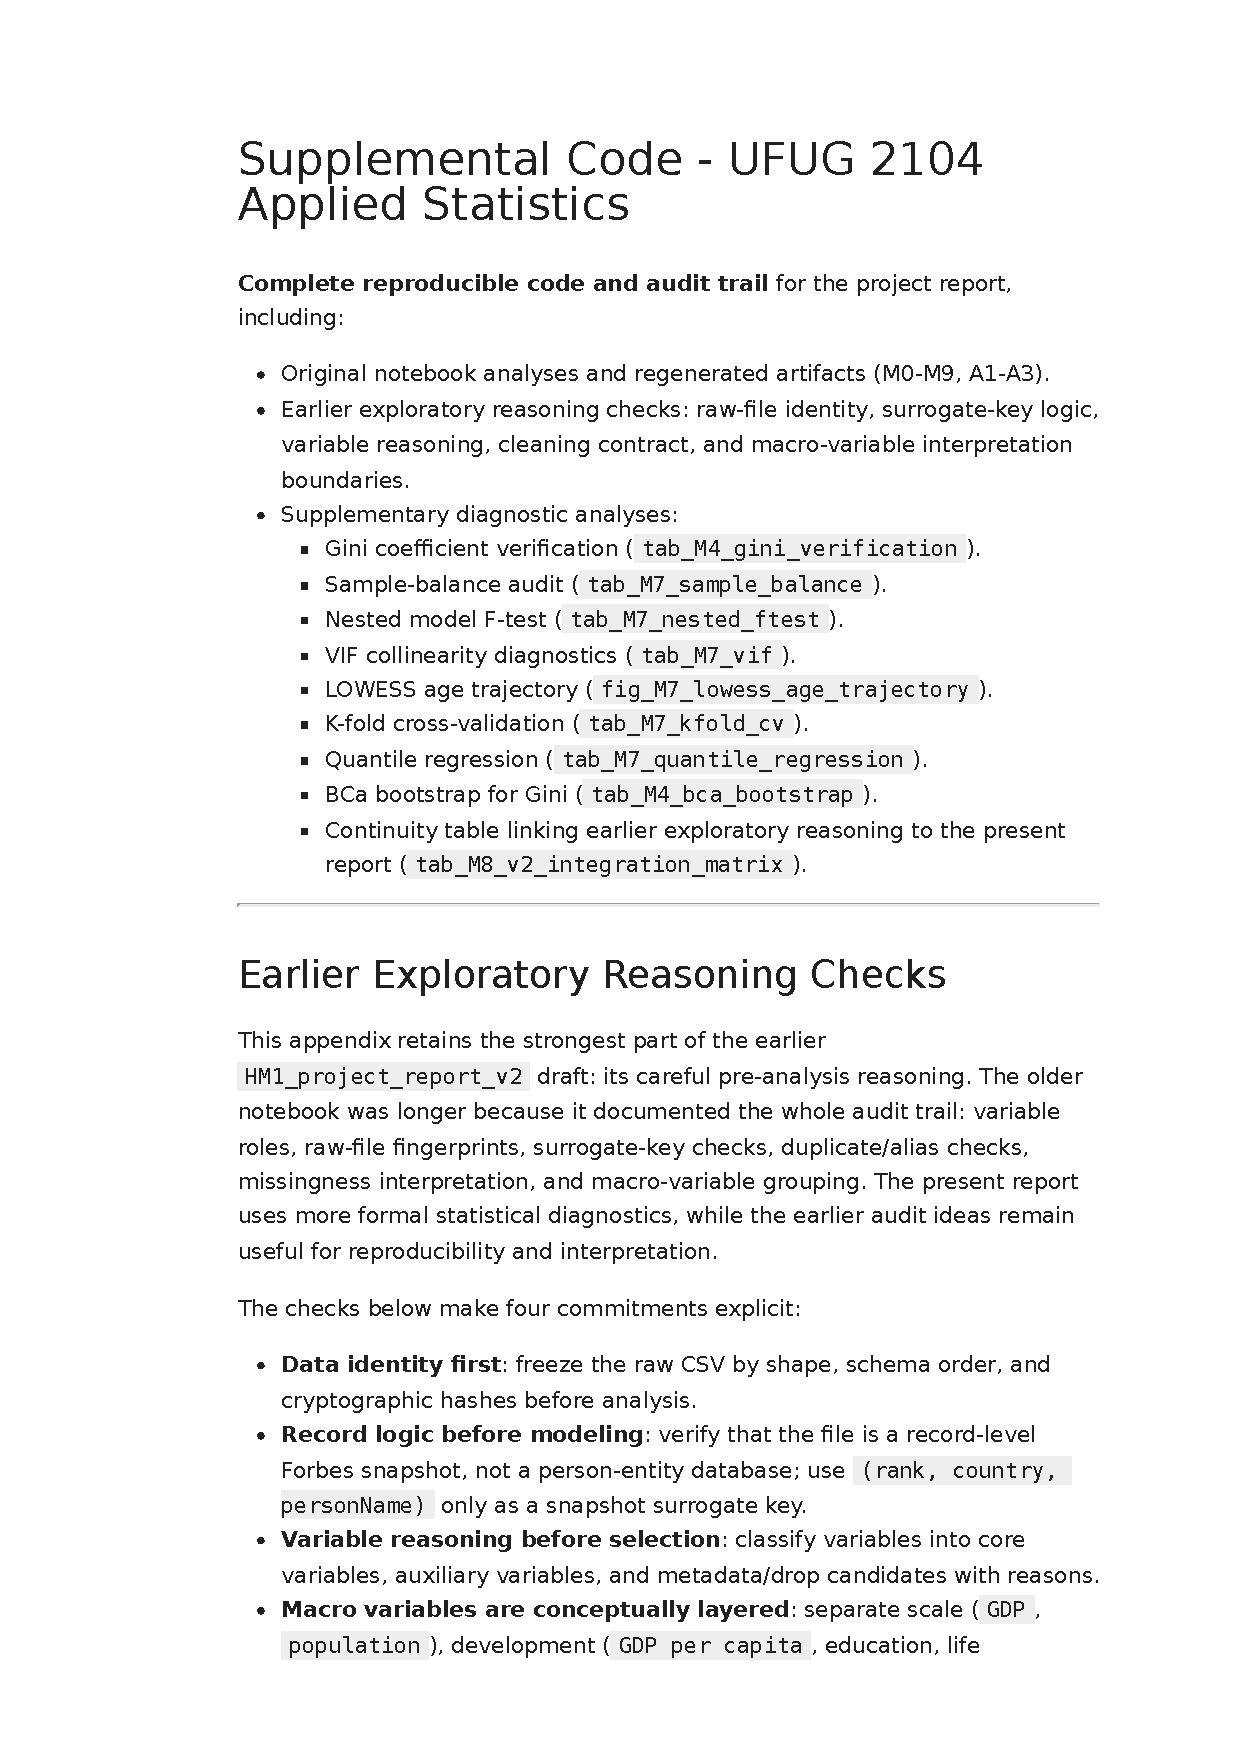
\includepdf[pages=-,fitpaper=true,pagecommand={}]{project_notebook.pdf}

\end{document}

